\chapter{A BCS-Josephson Wormhole in coupled superconducting Yukawa-SYK metals}
\label{chap:JosephsonWormhole}

\section*{Attribution}
The work in this chapter has been done jointly with Stephan Plugge and Koenraad Schalm, and is a manuscript under preparation.

% \begin{abstract}
\section*{Abstract}
\noindent
We show that two Yukawa-SYK models with a weak tunneling contact can have an exotic superconducting hybrid thermofield-double-like state holographically dual to a traversable wormhole connecting two black holes with charged scalar hair. 
% For strong tunneling this state crosses over to a conventional Josephson contact. 
The hybrid thermo-field-double/wormhole state is distinguishable by anomalous scaling of revival oscillations in the fermionic Green's function, while the BCS-like superconducting condensate is responseless. 
% This is a correlated with emergence of the superconducting state of Yukawa-SYK models emerges out of a quantum critical strange metallic normal state by the BCS-like opening of a gap \as{I'm not sure what the previous sentence is supposed to convey}. 
The existence of this TFD/wormhole state surprisingly shows that the some quantum critical effects can survive the phase transition to superconductivity. It also suggests a more strange metallic TFD/Josephson wormhole can exist correlated with superconductivity at strong coupling, where Cooper pairs persist above the critical temperature.
% \comment{DO YOU HAVE A FIGURE THAT SHOWS THE OPENING OF THE BCS GAP?}\as{no - I haven't had time to do the real time numerics including superconductivity}
% \comment{OK, Let's leave it to the reference to \cite{esterlis2021large} as we do now. Comment these comments out, when you agree.}
% \end{abstract}

%\keywords{Suggested keywords}%Use showkeys class option if keyword
                              %display desired
% \maketitle
%\tableofcontents

\section{Introduction}
\label{sec:introduction}

\noindent
The realization that the quantum critical strongly correlated groundstate of the Sachdev-Ye-Kitaev model 
%of disorder averaged interacting fermions 
is in the same universality class as the groundstate of holographic models of charged anti-de-Sitter black holes has opened up a wide avenue to study exotic gravitational questions with quantum-mechanical Hamiltonians. One such question is the existence of traversable wormholes. Maldacena and Qi \cite{maldacena2018eternal}, based on an earlier work of Gao, Jafferis and Wall \cite{gaoTraversableWormholesDouble2017} and more recently others \cite{maldacenaDivingTraversableWormholes2017,maldacenaTraversableWormholesFour2020,bakBulkViewTeleportation2018,gaoRegenesisQuantumTraversable2019,fuTraversableAsymptoticallyFlat2019,bakExperimentalProbesTraversable2019,qiCoupledSYKModel2020a,caceres2021sparse,haenel2021traversable,berenguer2024floquet},
%\comment{CHECK ALL/MORE}\as{done}, 
showed that (marginally) relevant tunneling interactions between two such SYK Hamiltonians could induce a phase transition to a finite temperature ``wormhole'' state as the temperature is lowered. The quantum mechanical understanding of this transition is as follows. At high temperatures, where tunneling is minimal, the state of the coupled system is arbitrarily close to two independent decoupled thermal ensembles at high temperature --- holographically dual to two black holes
\begin{align}
\label{eq:2BH-densitymatrix}
    \rho_{\text{2BH}} = \frac{1}{Z_{\beta}^2}\sum_{n_1,n_2} e^{-\beta (H_1+H_2)} |n_1,n_2\rangle\langle n_1,n_2|~.
\end{align}
The density matrix can also be written as a state in a doubled system
\begin{align}
\label{eq:2BH-state}
|\text{2BH}\rangle_{\beta} = \frac{1}{Z_{\beta}^2}\sum_{n_1,n_2} e^{-\beta (E_{n_1}+E_{n_2})} |n_1,\bar{n}_2\rangle~,
\end{align}
where $|\bar{n}\rangle = |\Theta n\rangle$ with $\Theta$ an anti-unitary symmetry of the SYK model (usually CPT).
As one lowers the temperature and the tunneling becomes stronger the thermodynamically preferred state is a different one. This is the state close to the maximally entangled so-called Thermo-Field-Double state --- holographically dual to a wormhole connecting the two black holes
\begin{align}
\label{eq:WH-state}
    |\text{WH}\rangle_{\beta} =|\text{TFD}\rangle_{\beta} = \frac{1}{\sqrt{Z_{\beta}}}\sum_n e^{-\frac{\beta}{2}E_{n}} |n,\bar{n}\rangle
\end{align}
Here $Z_{\beta}=\sum e^{-\beta E_n}$ is the partition function of a single SYK model.

Macroscopically it is a first order transition driven by the relevancy of the tunneling interaction, but the telltale sign of the wormhole is more subtle than a macroscopic order parameter. When the high temperature state is %still 
in the strongly correlated regime such that it is the finite temperature extension of the quantum critical SYK groundstate dual to a black hole, rather than a thermal gas of free quasiparticles, the low temperature ``wormhole'' state can remember this critical origin in that its spectrum can be better explained as a perturbation of its quantum critical spectrum rather than a perturbation around a free system. Specifically, the near-AdS$_2$ symmetry group (time-reparametrizations modulo $PSL(2)$) that defines the quantum critical state of a single SYK system, continues to determine the spectrum of the coupled system even when the groundstate changes to the TFD/WH state \cite{maldacena2018eternal}. This deformed N-AdS$_2$ spectrum has a uniquely characteristic fixed spacing between levels similar to that of a harmonic oscillator: $E_n = E_{\text{gap}}(1+ \frac{1}{\Delta}n), n \in \mathbb{N}$, with the groundstate energy $E_{\text{gap}}\sim \lambda^{\frac{1}{2-2\Delta}}$ proportional to a non-perturbative non-analytic fractional power of the tunneling strength $\lambda$ in terms of the IR critical scaling dimension $\Delta$ of a fermionic excitation. This fixed integer spacing in units of $c$ is observable in characteristic revivals in a linear response probe, as convincingly shown in subsequent numerical simulations \cite{maldacenaSYKWormholeFormation2020a,pluggeRevivalDynamicsTraversable2020a,sahoo_traversable_2020,qiCoupledSYKModel2020a}. %\comment{CHECK}\as{done}. 
From the dual holographic gravitational perspective this revival is a perturbation that has fallen into a black hole, traveled through the wormhole and back. One should be careful: Revival-signatures in linear response can have many origins and not all revivals are dual to a signal traversing a wormhole. The key aspect is the non-analytic dependence of the gap $E_{\text{gap}}$ and the spacing $\Delta E =E_{\text{gap}}/\Delta$ on the relevant tunneling strength $\lambda$. Even within these SYK-models, if this relevant coupling becomes strong, the system still shows revivals. But as the system has now crossed over to a free-fermion state, the gap and the level spacing underlying the revivals are now an integer analytic power of tunneling strength. It is just a reflection of the regularity of the underlying standard free particle harmonic oscillator spectrum. 
Fig.\ref{fig:Schematic Phase diagram}A summarizes this phase diagram of the 2BH/WH transition in quantum critical SYK models.




However theoretically appealing, in actual physical systems quantum critical states are rare. Moreover, experimentally they are fragile and extremely susceptible to decay to a conventional ordered state, usually a BCS superconductor. It is conjectured that in 2D systems this is in fact always the case \cite{metlitskiAreNonFermiliquidsStable2015,abanov2020interplay,chubukov2020interplay}.
The SYK-like quantum critical systems are essentially 0D quantum dots, but 2D extensions can preserve many of its features including the N-AdS$_2$ like structure of its groundstate \cite{patel2023universal}. Some of the fragility of this quantum critical grounstate is suppressed by a large $N$-limit, but some is also by construction. In particular the simplest SYK models do not preserve time-reversal symmetry and singlet Cooper pairs are not stable enough to form a long range coherent state. More realistic models must preserve (some) time reversal symmetry to allow pairing. One such model is the Yukawa-SYK model constructed in \cite{esterlis2019cooper}. This is a quantum critical superconductor with a tunable pairing strength and $T_c$ whose condensate is not controlled by the density of states at the Fermi surface \cite{sheBCSSuperconductivityQuantum2010,esterlis2019cooper}. 
%\comment{CHECK FIRST REFERENCE.}\as{done} 
In particular, the charge neutral critical state with no Fermi surface is already unstable towards superconductivity. It is able to do so as the density of states is large even at charge neutrality, which allows a macroscopic condensate to form.
%\comment{CHECK}
For a large part of the phase diagram this superconductivity indeed prevents the emergence of quantum criticality, but this view has been challenged recently in Ref.~\cite{zhang2023density}.


The question we address in this article is whether the exotic revival physics dual to a wormhole state persists in tunneling contacts between such more realistic SYK models as Yukawa-SYK that do exhibit superconductivity. Naively one would think not, in accordance with the wisdom that superconductivity prevents quantum criticality. The onset of superconductivity gaps the low-energy spectrum and this ought to destroy to characteristic fixed level spacing responsible for the wormhole revival physics. The loophole is that in these models superconductivity is tunable and a window may exist that nevertheless allows for a sufficiently regular spectrum that a wormhole like state survives. The holographic gravitational dual of such a state would be a wormhole with a scalar condensate also known as scalar hair. An argument in favor that such state could result from this construction is the fact that the thermofield-double state is a formal purification of the straightforward thermal mixed state of a single YSYK model. It must therefore exist, and perhaps the better posed question is whether this protocol contructs the TFD-state as the groundstate of the coupled YSYK system.      

In this article we report that this indeed turns out to be the case and the loophole is realized --- in a particular way. There exists indeed a strongly entangled tunneling contact state between two superconducting YSYK systems that nevertheless has a low-energy spectrum controlled by the N-AdS$_2$ of the critical state. Pictorially this is represented in Fig. \ref{fig:Schematic Phase diagram}B.
The particularity of this state is that the regime where this state is found is one where superconducivity manifests itself in the fermionic spectrum by the BCS-like opening of gap. Qualitatively, this means that Cooper pairs condensate immediately upon binding and there are no uncondensed bound-fermion states in the spectrum. 
%In effect the TFD/wormhole state is not given by Eq.~\ref{eq:WH-state}, but by a state close to \comment{BETTER NAME}
%\begin{align}
%    |\text{partial}-WH\rangle_{\beta} = |\text{partial}-TFD\rangle_{\beta} = \frac{1}{Z_{\beta}} \sum_n_F e^{-\frac{\beta}{2}}|n_F,\bar{n}_F\rangle\otimes|0,0\rangle
%\end{align}
The ``wormhole'' state is therefore the honest TFD of the fermionic excitations on top of the BCS-like groundstate. This is in contrast to a more BEC-like superconductivity where bound states form first, exist as independent asymptotic excitations in the spectrum, and only condense at a lower temperature. In the fermionic spectral function this manifests itself as a depletion of the gap/growth of a peak at finite energy, as is observed in real high $T_c$ strange metals for instance \cite{kondoPointNodesPersisting2015,reberPairingPairbreakingTheir2015a,liCoherentOrganizationElectronic2018,bastiaansDirectEvidenceCooper2021,trompPuddleFormationPersistent2023}. The TFD/``wormhole'' state of such a system would have the same formal form as Eq.~\eqref{eq:WH-state}, but now the energy states would contain both fermionic and bosonic excitations. In principle the YSYK model we study has a regime where such BEC-like superconductivity occurs \cite{esterlis2019cooper}. However, generically this originates from an impurity-like normal state above $T_c$ and not from the quantum critical state holographically dual to black holes. We have therefore not studied this here.

Tunneling contacts between superconducting systems --- a Josephson junction --- are of course an enormously well studied and useful arena of physics. As the Josephson current is the tunneling of Cooper pairs, an immediate question is whether the %AC 
Josephson current can also show revivals characteristic of a ``wormhole''. 
Even if quantum in origin, the dominant Josephson effects are macroscopic thermodynamic manifestions: they are captured by the Landau-Ginzburg free energy. The universality of the latter precludes any significant change in observational responses due to an underlying TFD/wormhole state. We confirm this by a computation of the DC Josephson current in the TFD/wormhole state. Similar to non-superconducting SYK models, the manifestation of the wormhole is more subtle. A more fine grained analysis of Josephson physics may reveal other effects in addition to the single fermion revivals. We leave this for further study. 
%\comment{[DROP? BETTER NAME?]}
Nevertheless, as the superconductor-superconductor wormhole is supported by a tunneling interaction, to christen it the BCS-Josephson wormhole seems apt.



Section \ref{sec:model} describes the YSYK model, the tunneling interaction coupling two YSYK models and the effective Schwinger-Dyson equations controlling the large $N$-limit of the model after disorder averaging over random four-fermion interactions. Section \ref{sec:metallic-state} describes the TFD/wormhole state when superconductivity is artifially surpressed to connect with earlier coupled SYK wormhole results and set the stage for Section \ref{sec:sc-state} where we exhibit the existence of the BCS-Josephson wormhole, i.e. a thermodynamic phase transition to a superconducting TFD-state. From the free energy of the total system we compute the DC Josephson current to show that it is not affected by the underlying state change as could have been surmised by the fact that the TFD-state is thermodynamically in the same phase as the ordinary BCS state. We conclude with a brief outlook in the conclusion Section \ref{sec:conclusion}.


%To answer this requires a more detailed analysis than we present in this paper. We can, however,


\begin{figure}[t]
    \centering
    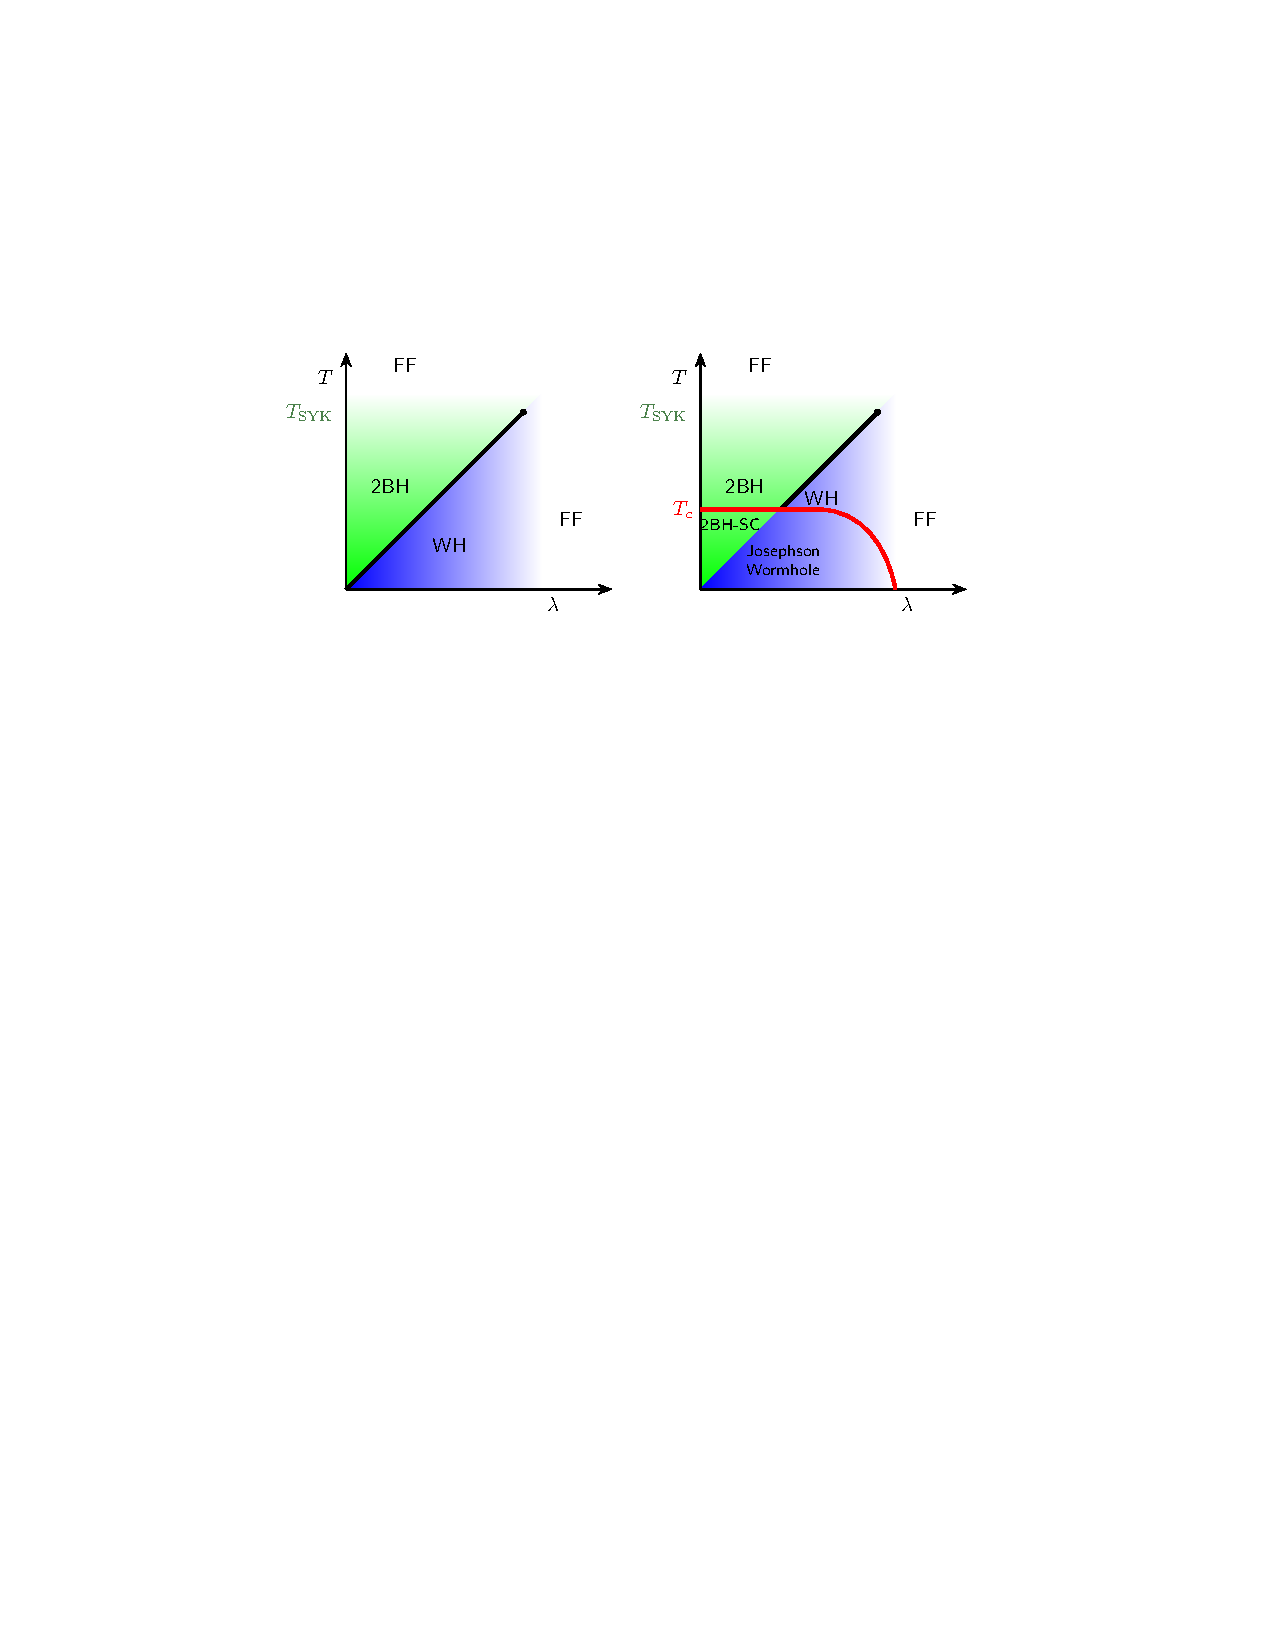
\includegraphics[width=0.9\linewidth]{figures/chapter3/2YSYK-PhaseDiagram-v3.pdf}
    \caption{
        Schematic phase diagram of two coupled Yukawa-SYK systems without (left) and with superconductivity (right). When superconductivity is suppressed, there is a first order phase transition at fixed $\lambda < \lambda_{\text{SYK}}$ for $T\sim \lambda$. There the system transitions from a intermediate temperature $T\lesssim T_{\text{SYK}}$ state of essentially two decoupled thermal strongly correlated SYK systems holographically dual to two black holes (2BH), to a low temperature thermofield double state with specific cross-correlations holographically dual to wormhole (WH).  At very high temperatures $T \gg T_{\text{SYK}}$ or very high tunneling coupling $\lambda\gg\lambda_{\text{SYK}}$ the coupled system is in a free fermion phases that are smoothly connected to each other. When superconductivity is included. The above is valid for an intermediate value of the averaged Yukawa-YK-coupling in terms of the bare boson mass $g_{\text{SYK}}/\omega^{3/2}\sim 0.5$, the two-black-hole phase first becomes a two essentially independent superconductor phase, holographically dual to two hairy black holes (2BH-SC). This state crosses over around the value of the putative 2BH/WH phase-transition to a excitation spectrum on top of the superconducting groundstate that is characteristic of the thermo-field-double/wormhole state.  %On lowering the temperature, we find first powerlaw correlations developing in the diagonal green's function. We call this non-fermi liquid state (NFL) which is dual to a two sided black hole geometry. At the lowest temperatures however, i.e. when $T \ll \lambda $, the system undergoes a first order transition to the wormhole state. The two phases are demarcated by a line $T \sim \lambda$. 
        %\comment{Include $T_{\text{SYK}}\sim g^{2/3}$ DONE; ALSO EDITED}
        }
    \label{fig:Schematic Phase diagram}
\end{figure}
%\comment{
%\begin{itemize}
%    \item {\bf Characteristics}
%    \item Josephson current
%    \comment{(four point function?)/Numerics}
%    \item 
%\end{itemize}
%}




%##################

\section{Two Yukawa-SYK models with a tunneling contact with shared disorder.}
\label{sec:model}

\noindent
The Yukawa-SYK model describes a quantum dots with $N$ flavors of spin-$\frac{1}{2}$ fermions and $M$ flavors of bosons with Hamiltonian \cite{esterlis2019cooper}
\begin{align}
       H_{\text{Y-SYK}} = -\mu\sum_{i=1}^N\sum_{\sigma=\uparrow,\downarrow} c^\dagger_{i,\sigma} c^{\phantom{\dagger}}_{i, \sigma} + \sum_{k=1}^M \frac{1}{2}\left(\pi_k^2 + \omega_0^2\phi_k^2\right) + \frac{\sqrt{2}}{N}\sum_{i,j,k}\sum_{\sigma}g_{ijk} c^\dagger_{i,\sigma} c^{\phantom{\dagger}}_{j,\sigma} \phi^{\phantom{\dagger}}_k~.
    \label{eq:HYSYK}
\end{align}
In a single instance of the model the complex couplings $g_{ijk}=g^{'}_{ijk}+ig^{''}_{ij,k}$ are randomly drawn from an ensemble with zero mean and variance
\begin{align}
    \langle g'_{ijk}g'_{lmn}\rangle &= (1-\frac{\alpha}{2})g^2\delta_{kn}(\delta_{il}\delta_{jm}+\delta_{im}\delta_{jl})~,\nonumber\\
    \langle g''_{ijk}g''_{lmn}\rangle &= \frac{\alpha}{2}g^2\delta_{kn}(\delta_{il}\delta_{jm}-\delta_{im}\delta_{jl})~,\nonumber\\
    \langle g'_{ijk}g''_{lmn}\rangle &=0~.
\end{align}
For $\alpha=1$ the hermitian matrix $g_{ijk}=(g_k)_{ij}$ is in the Gaussian Unitary ensemble; for $\alpha=0$ the matrix is real and in the Gaussian orthogonal ensemble. The model is solvable after averaging over the ensemble and taking the double limit $N\rightarrow \infty$, $M\rightarrow\infty$ with $\kappa=M/N$ fixed.
For $\alpha=1$ the system has a quantum critical SYK groundstate for any value of the chemical potential $\mu$ and boson mass $\omega_0$ with scaling dimensions $\Delta_f$ and $\Delta_b$ for the fermions and bosons respectively that are fixed by 
%Upon starting from the high temperature phase FF1 and lowering temperature below the scale $T_{SYK}$, we see the onset of the NFL state and its emergent conformal symmetry. At low frequencies, the diagonal Green's functions scale with a power law 
% \begin{align}
%     G(\omega) &\sim \abs{\omega}^{2\Delta_f-1}\sgn(\omega) \\
%     D(\omega) &\sim \abs{\omega}^{2\Delta_b-1} \,.
%     \label{eq:scalingsolns}
% \end{align}
% In these equations, $\Delta_f$ and $\Delta_b$ are the scaling dimensions of the fermions and bosons respectively, and can be calculated in the conformal limit of the Schwinger-Dyson equations. They need to satisfy
\begin{align}
\label{eq:YSYK-scaling-dims}
    2\Delta_f + \Delta_b &= 1 \, ,\non
    \kappa\frac{\Gamma(1-\Delta_f)\Gamma(1-(\Delta_f+\Delta_b))}{\Gamma(\frac{1}{2}+\Delta_f)\Gamma(\frac{1}{2}+\Delta_f+\Delta_b)} &= -2 \frac{\Gamma(\frac{1}{2}-\Delta_b)\Gamma(\frac{1}{2}-2\Delta_f)}{\Gamma(\Delta_b)\Gamma(2\Delta_f)} .
\end{align}
(see Appendix \ref{app:effectiveaction}). For $\alpha < 1$ the theory has a time-reversal preserving sector and allows for pairing and a stable superconducting phase. In particular, at $\alpha=0$ for a small range of $g \sim \omega_0^{3/2}$ the phase diagram (Fig.~\ref{fig:YSYK-phase-diagram}) has a small window where the onset of superconductivity occurs from the finite temperature extension of the quantum critical Yukawa-SYK N-AdS$_2$ state holographically dual to a black hole~\cite{esterlis2019cooper,wang2020solvable,classen2021superconductivity,inkof2022quantum}. We shall choose the model with $\alpha=0$ at charge neutrality $\mu=0$ with that value of $g/\omega_0^{3/2}=0.5$ and hold these fixed throughout this study; we shall also choose $\kappa=1$ throughout.
%\comment{CHECK}\as{correct}
What shall be important later in Section \ref{sec:sc-state}, is that for this value the onset of superconductivity manifests itself in the fermionic spectral function by the opening of a gap (Fig.~6 in \cite{esterlis2019cooper}), i.e. bound fermion states immediately condense and the spectrum of excitations does not contain bound-fermion states.
%\comment{CHECK}\as{correct}.

\begin{figure}[t!]
    \centering
    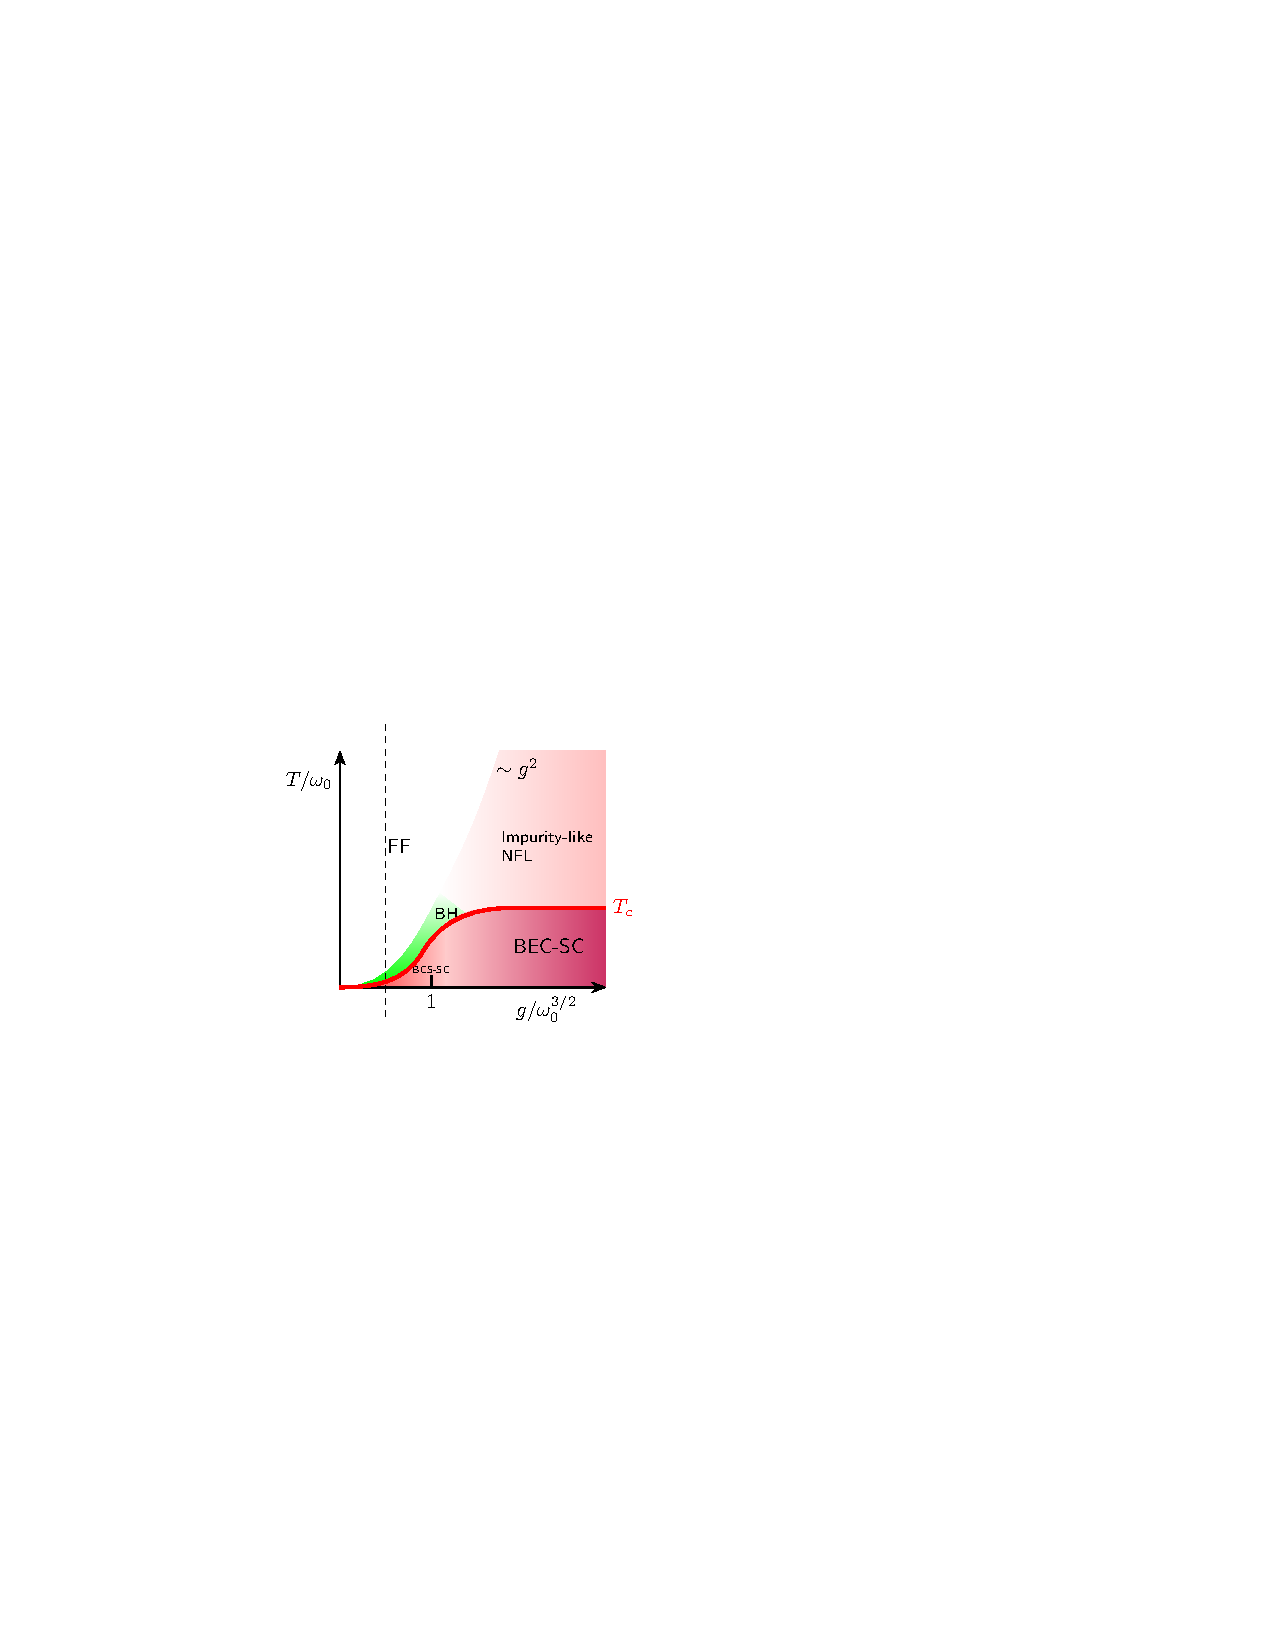
\includegraphics[width=0.5\linewidth]{figures/chapter3/YSYK-PhaseDiagram-v3.pdf}
    \caption{The phase diagram of a single Yukawa-SYK model with couplings drawn from the GOE from \cite{esterlis2019cooper}. FF is a free-fermion phase; BH is the finite temperature version of the quantum critical N-AdS$_2$ SYK groundstate dual to a black hole. SC is the superconducting state which has a crossover from BCS-like SC to BEC-like SC as $g/\omega_0^{3/2}$ increases. At high temperatures for large $g$ the model is controlled by an impurity fixed point. 
    The dashed line denotes the value of the disorder-averaged coupling $g/\omega_0^{3/2}=0.5$ we use in this in article such that the normal phase right above the superconducting transition is the quantum critical/BH phase.}
    \label{fig:YSYK-phase-diagram}
\end{figure}

The two coupled system configuration that allows for entangled TFD phase at low temperatures is constructed by coupling two identical Yukawa-SYK models, i.e. with the same random coupling constants {\em before disorder averaging}, together with a simple tunneling interaction.
% \begin{align}
%     H=H_{\text{YSYK}}^{(1)}[g_{ijk}] + H_{\text{YSYK}}^{(2)}[g_{ijk}] + \sum_{i,\sigma} \lambda c^{\dagger(1)}_{i\sigma}c^{(2)}_{i\sigma} +\lambda^\dagger c^{\dagger(2)}_{i\sigma}c^{(1)}_{L,i\sigma}~.
% \end{align}
%$
% are disorder-averaged 
% on each of them respectively, and described separately by the Yukawa SYK Hamiltonian, with exactly the same realization of disorder on each side. We are interested in this model in the of large fermion and boson flavors $M\rightarrow\infty$, $N\rightarrow\infty$, such that the ratio $\kappa = \nicefrac{M}{N}$ is constant.
%The two individual dots are then coupled by a fermion interaction across the two dots, of strength $\lambda$. 
The joined model is then described by the following action
% \begin{widetext}    
\begin{align}
    S &= S^{(1)}[g_{ijk}] + S^{(2)}[g_{ijk}] + S_c \, , \nonumber \\
    S^{(a)}[g_{ijk}]&= \int \!\dd\tau \sum_{i,\sigma} {c^\dagger}^{(a)}_{i\sigma}(\tau) \left(\partial_\tau - \mu\right)c^{(a)}_{i\sigma}(\tau) + \sum_k \phi^{(a)}_k(\tau)\frac{1}{2}\left(-\partial_\tau^2 + \omega_0^2\right) \phi^{(a)}_k(\tau) \nonumber\\
     &~~~~~~+ \frac{\sqrt{2}}{N}\int\!\dd\tau \sum_{ijk,\sigma} g_{ijk}{c^\dagger}^{(a)}_{i\sigma}(\tau)c^{(a)}_{j\sigma}(\tau)\phi^{(a)}_k(\tau) \, ,\nonumber\\
    S_c &= \int \!\dd\tau \sum_{i,\sigma}\lambda {c^\dagger}^{(1)}_{i\sigma}(\tau)c^{(2)}_{i\sigma}(\tau) + \lambda^* {c^\dagger}^{(2)}_{i\sigma}(\tau)c^{(1)}_{i\sigma}(\tau) 
    %+ \sum_k J\phi^{(1)}_k(\tau)\phi^{(2)}_k(\tau) \,.
    \label{eq:bareaction}
\end{align}
% \end{widetext}
% In what follows, we will refer to the two dots with indices $(1,2)$ or $(L,R)$ respectively, and refer to the system as the two-sided Yukawa SYK model. 
%
% The $g_{ijk}$ are in general random complex numbers, but they are all not independent, and have constraints imposed by requiring that the hamiltonian be hermitian. In the absence of time-reversal symmetry (TRS), the couplings $g_{ijk}$ would be drawn from the Gaussian Unitary ensemble (GUE). When TRS is present however, the couplings would need to be drawn from the Gaussian Unitary ensemble (GUE). 
Other tunneling couplings such as boson-boson tunneling $S=\int\dd\tau J\phi^{(1)}_k\phi^{(2)}_k$ or correlated two-fermion tunneling $S=\int\dd\tau g_{ijk}g_{lmk} {c^\dagger}^{(1)}_{i\sigma}(\tau)c^{(2)}_{j\sigma}(\tau) c^{\dagger(1)}_{k\sigma'}c^{(2)}_{l\sigma'} +\text{c.c.}$ are possible. By dimensional analysis, such terms are less relevant in the IR. As a similar study for complex SYK models has shown \cite{sahoo_traversable_2020}, there is still a transition to a TFD/wormhole state, but is weaker, at lower temperature and harder to detect. Moreover, such boson-boson and correlated multi-fermion tunnelings are also dynamically generated at subleading order in $\lambda$. We will therefore not consider such couplings here. 

%The coupled theory has an overall $U(1)$ symmetry as well as a discrete swap symmetry $c_1 \rightarrow c_2e^{i\theta}, ~c_2 \rightarrow c_1 e^{-i\theta}$ where $\theta$ is the phase of the tunneling coupling $\lambda=|\lambda|e^{i\theta}$. We shall use this symmetry later in discussing the Josephson physics.
% In the rest of the article, we will work with $g=0.5$ and at the charge neutrality point $\mu=0$. These parameters are chosen so that the finite temperature state of the one-sided model exhibits only the NFL phase and not the impurity phase~\cite{esterlis2019cooper}. For convenience, we will also set $J=0$ and study the model only with the bare fermion cross coupling $\lambda$ explicitly introduced. It can be noted that a coupling between the bosons on the two sides will be dynamically generated through a fermion mediated mechanism.

The coupled system is solved by disorder averaging over the couplings $g_{ijk}$ that are identical in subsystem $(1)$ and $(2)$ in each instance of the ensemble.
Introducing bilocal fields 
\begin{align}
    G^{ab}(\tau,\tau') &=-\frac{1}{N} \sum_i\cind{a}{i}{\tau}\cdag{b}{i}{\taup} \nonumber\\
    F^{ab}(\tau,\tau') &=-\frac{1}{N}\sum_i\cind{a}{i}{\tau}\cind{b}{i}{\taup}\nonumber\\
    D^{ab}(\tau,\tau') &=-\frac{1}{M}\sum_k\phi^{(a)}_k(\tau)\phi^{(b)}_k(\taup).
\end{align}
through their respective self-energies $\Sigma_{ab}, \Phi_{ab}, \Pi_{ab}$ as Lagrange multipliers, one can perform the path-integral over the fermions. The resulting effective action in terms of these bilocal fields has a set of Schwinger-Dyson equations as saddle-point equations. Using the fact that the original action Eq.\eqref{eq:bareaction} has a $\mathbb{Z}_2$ mirror symmetry $c_1 \rightarrow c_2e^{i\theta}, ~c_2 \rightarrow c_1 e^{-i\theta}$ where $\theta$ is the phase of the tunneling coupling $\lambda=|\lambda|e^{i\theta}$, the large $N,M$ saddle-point Schwinger-Dyson equations can be expressed in terms of $G_{d} = G_{11}= G_{22}, G_{od} = G_{12} = e^{2i\theta} G_{21}$ etc only. Assuming time-translation invariance in addition, they are %The Euler-Lagrange equations for the $G$-variables are easy to obtain and they can be written as: 
%
\begin{align}
     \Sigma_{ab}(\tau,\taup) &= \kappa g^2 D_{ab}(\tau,\taup)G_{ab}(\tau,\taup)\,,
     \non
     \Phi_{ab}(\tau,\taup) &=  -(1-\alpha)\kappa g^2 F_{ab}(\tau,\taup) D_{ab}(\tau,\taup)\,,
     \non
     \Pi_{ab}(\tau,\taup) &= -2 g^2\left[
     G_{ab}(\tau,\taup)G_{ba}(\taup,\tau)
     -(1-\alpha)F_{ab}(\tau,\taup)\Bar{F}_{ba}(\taup,\tau)\right]\,,\non 
\begin{pmatrix}G_{11} & F_{11} & G_{12} & F_{12} \\
\bar{F}_{11} & \tilde{G}_{11} & \bar{F}_{12} & \tilde{G}_{12} \\
G_{21} & F_{21} & G_{22} & F_{22} \\
\bar{F}_{21} & \tilde{G}_{21} &\bar{F}_{22} & \tilde{G}_{22}
\end{pmatrix} &= \mqty(i\omega_n-\Sigma_{11} & -\Phi_{11} & -\lambda - \Sigma_{12} & -\Phi_{12} \\ -\bar{\Phi}_{11} & i\omega_n - \tilde{\Sigma}_{11} & -\bar{\Phi}_{12} & \lambda^\ast - \tilde{\Sigma}_{12} \\ -\lambda^\ast - \Sigma_{21} & -\Phi_{21} &i\omega_n-\Sigma_{22} & -\Phi_{22} \\ -\bar{\Phi}_{21} & \lambda - \tilde{\Sigma}_{21} & - \bar{\Phi}_{22} & i\omega_n - \tilde{\Sigma}_{22})^{-\top}\, , \non
    \begin{pmatrix}
    D_{11}(i\nu_n) & D_{12}(i\nu_n)  \\
    D_{21}(i\nu_n)  & D_{22}(i\nu_n) 
    \end{pmatrix}&= \mqty(\nu_n^2+\omega_0^2-\Pi_{11}(i\nu_n)  & \Pi_{12}(i\nu_n)  \\
    \Pi_{21}(i\nu_n)  & \nu_n^2 + \omega_0^2 - \Pi_{22}(i\nu_n) )^{-\top} \,.
\end{align}
%Where $\hat{G}$ is a matrix such that it's $ij^{\text{th}}$ element contains the normal/anomalous fermion Green's function whose corresponding self energy appears in the $ij^{th}$  component of the matrix on the right, and likewise for the matrix $\hat{D}$ for the bosons. 
%\comment{WHAT IS $\tilde{G}, \tilde{\Sigma}$}
Here $\tilde{G}(i\omega_n)=-G^\ast(i\omega_n)$ is the Green's function for spin down fermions in the Nambu basis.
%, with $\tilde{G}(i\omega_n) = -G^\ast(i\omega_n)$. 
%\comment{I DO NOT UNDERSTAND IS. I EXPECT A RELATION LIKE $\tilde{G}=G\star$ OR TIME-REVERSED OR SOMETHING.}\as{That was a typo - I put $\Sigma$ earlier where there should have been a $G$. Now fixed.}
%where 
In the fermionic matrix equation all self energies are evaluated at the Matsubara frequencies $\Sigma_{ab}(i\omega_n), \Phi_{ab}(i\omega_n)$.
Details of the derivation are given in the appendix~\ref{app:effectiveaction}. 



%#
\section{The YSYK-TFD/wormhole for the metallic normal state}
\label{sec:metallic-state}
%
%
% Since the two sided action in appendix~\ref{app:effectiveaction} explicitly couples the different copies, one cannot impose a replica symmetric action as is usually done in the SYK literature. However, an additional symmetry can be used to reduce the number of Green's functions one needs to keep in the computations. 
% We observe symmetry upon swapping the two layers. 
% \begin{align}
%     c_1 &\rightarrow c_2 e^{i\theta}\\
%     c_2 &\rightarrow c_1 e^{-i\theta} \\
%     \phi_1 &\leftrightarrow \phi_2  
%     \label{eq:mirror_symmetry}
% \end{align}
% leaves the action invariant: this is the definition of mirror symmetry for this case. The point is that no matter what phase the complex coupling $\lambda$ has, we can pick $\theta$ appropriately for the symmetry to hold. Thus, we can make a gauge choice $\lambda$ to be purely real, giving $\theta = 0$. This leaves, $G_{11}=G_{22}=G_d$ and $G_{12} = G_{21} = G_{od}$. This is the convention we will stick to in what follows. As a side remark, notice that if we had picked as a gauge choice $\lambda$ to be purely imaginary, we would have had $G_{11} = G_{22}$ and $G_{12} = -G_{21}$. 
% %

To show that the N-AdS$_2$ quantum critical point of the time-reversal symmetry breaking non-superconducting version of the YSYK model has a TFD/wormhole state in the weak tunneling configuration of two coupled systems, we first study the coupled system with superconductivity suppressed. It is metallic for all temperatures. For this we set $\alpha=1$ which breaks time-reversal symmetry completely. 
The Schwinger-Dyson equations simplify to 
\begin{align}
    \det G &= (i\omega_n + \mu -\Sigma_d)^2 - (\lambda + \Sigma_{od})^2 \non
    G_d(i\omega_n) &= \frac{i\omega_n + \mu -\Sigma_d}{\det G}\non
    G_{od}(i\omega_n) &= \frac{(\lambda + \Sigma_{od})}{\det G} \non
    \det D &= (\nu_m^2 + \omega_0^2 - \Pi_d)^2 - (\Pi_{od})^2 \non
    D_d(i\nu_m) &= \frac{\nu_m^2 + \omega_0^2 - \Pi_d(i\nu_m)}{\det D} \non
    D_{od}(i\nu_m) &= \frac{\Pi_{od}}{\det D}\non
    \Sigma_{(o)d}(\tau) &= \kappa g^2\, D_{(o)d}(\tau) G_{(o)d}(\tau)\non
    \Pi_{(o)d}(\tau) &= -2 g^2\, G_{(o)d}(\tau)G_{(o)d}(-\tau)
    \label{eq:SDeqnsmetal}
\end{align}
%
Note from the last two equations that the interacting part of the Schwinger-Dyson equations for the off-diagonal components is just a copy of the interacting part of the Schwinger-Dyson equations for the diagonal part and that they do not mix.
%The functional dependence of the self energies on the boson and fermion Green's functions at the saddle point is the same as the single dot Yukawa-SYK model for the diagonal and off-diagonal components separately. 
%\comment{What does the previous sentence mean?}\as{fixed} 
%\comment{REPHRASED AGAIN. CHECK}\as{checked - fixed a minor typo}. 
These equations can be solved numerically in imaginary time and Matsubara frequency.

%\section{The Phase diagram of the tunneling coupled YSYK system}

We first delineate the phase diagram of the coupled metallic $\alpha=0$ YSYK system as a function of $T$ and the coupling strength $\lambda$ already sketched in Fig.~\ref{fig:Schematic Phase diagram}A.
%The phase diagram of the non-superconducting state in the $T-\lambda$ plane contains two free fermion limits, when the scale $T_{SYK}$ is not the dominant one as is represented in Fig.~\ref{fig:Schematic Phase diagram}. 
%
At high temperature, when $T \gg T_{SYK}\sim g^{2}/\omega_0^2$ 
%\comment{CHECK UNITS}\as{checked} 
for any $\lambda$ the system is in a nearly free fermion phase, where the interactions $g$ and tunneling $\lambda$ only give small perturbative corrections to the free fermion Fermi-Dirac density matrix state. The diagonal Green's function is well approximated by $G_{d}(\tau)\sim -\frac{1}{2}\sgn(\tau)$ at small time scales.  Correspondingly, $G_{d}(i\omega_n) \sim \frac{1}{i\omega_n} $. as seen in the high frequency tail of the inset in Fig.~\ref{fig:GreenFunctionPlotsMetalv2}. 
%\comment{Figure?}\as{done} 
This represents the situation in which the fermions are essentially separately free in each dot.

For very large $\lambda$ this phase continues to extend to lower temperatures as well. For $\lambda \gtrsim g^{2}/\omega_0^2$ the tunneling coupling is more dominant and essentially acts as an ``off-diagonal'' mass term between the two systems. After diagonalization one expects a gapped state with $E_{\text{gap}}\sim \lambda$ and this gap prevents a flow to a quantum critical state. The diagonal Green's function shows this gap 
and has a long time behavior for $\frac{1}{E_{\text{gap}}} \lesssim \tau \lesssim \beta$ 
%\comment{check: units don't work. I think you mean $\frac{1}{E_{\text{gap}}} \lesssim \tau \lesssim \beta$ CHECK} \as{yes - the time range $\frac{1}{E_{\text{gap}}} \lesssim \tau \lesssim \beta$ is correct} 
that, as behoves a nearly free fermion system, is 
%can be seen in the 
%The other free fermion phase FF2 is seen when $\nicefrac{T}{\lambda}\ll 1$ and $\lambda, T \gg T_{SYK}$ the diagonal Green's function is 
well approximated by turning off the self-energies in Eq.~\eqref{eq:SDeqnsmetal} %and taking the limit of zero temperature, so that 
%\comment{Figure?}\as{Added Fig.\ref{fig:LargeLambdaGapScaling}}
\begin{align}
    G_d^0(\tau) &= \int_{-\infty}^{\infty} \frac{d\omega}{2\pi}\, \frac{i\omega}{(i\omega)^2 - \lambda^2} \nonumber \\
    &= -\frac{1}{2}\sgn(\tau) e^{-\lambda\abs{\tau}}.
    \label{eq:Gd0taulambda}
\end{align}
See Fig.~\ref{fig:LargeLambdaGapScaling}.
This represents a situation when the fermions just occupy the ground state of the cross coupling part of the hamiltonian, but are otherwise free. When analytically continued to the real axis, the spectral function would simply represent a quasiparticle pole at $\pm\lambda$.
\begin{figure}
    \centering
    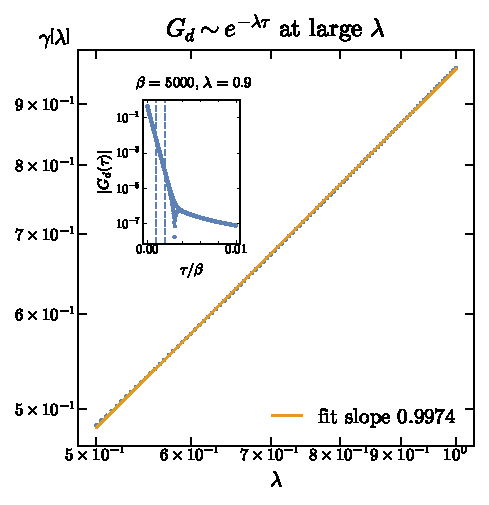
\includegraphics[width=0.8\linewidth]{figures/chapter3/LARGElambdalinearscaling.pdf}
    \caption{For large $\lambda \gtrsim g^{2}/\omega_0^2$, 
    %\comment{THIS FOLLOWS FROM THE FACT THAT THE PHASE TRANSITION IS AT $T\sim\lambda$ AND $T_{SYK}=g^{2/3}$. IS THE LATTER CORRECT? COULD ALSO BE $\lambda \gtrsim g/\omega_0^{1/3}$ CHECK. I THINK EITHER IS MORE CORRECT THAN $\lambda \sim \omega_0$} \as{agreed, $g^{2/3}$ is better. Esterlis and Schmalian in Ref.~\cite{esterlis2019cooper} use $T_{SYK} = \frac{g^2}{\omega_0^2}$, but I think $g^{2/3}$ is also good. NOTE: what they call $\bar{g}$ is $g$ for us.}\comment{OK, WE SHOULD CORRECT THIS TO ESTERLIS.},
    the diagonal fermion Green's function has a gap that scales linearly with $\lambda$, and is well approximated by Eq.~\ref{eq:Gd0taulambda}.}
    \label{fig:LargeLambdaGapScaling}
\end{figure}
%
Formally this is the same phase as the high temperature phase as it simply the irrelevance of mass at high temperatures as is reflected in the smooth deformation of the one Green's function into the other. 
%and indeed the FF2 form of the diagonal Green's function becomes the FF1 form in the limit of $\lambda\rightarrow 0$.

At small $\lambda \lesssim g^{2}/\omega_0^2$ there are different phases. 
%and their results are shown in Fig.~\ref{fig:GreenFunctionPlotsMetal}. In imaginary time the Green's functions are periodic and we show only half the period --- the full periodicity is shown in the inset.
%
%\subsection{Free fermion phases}
Now the YSYK coupling $g$ is more important.
From dimensional analysis, it can be expected to become important at an energy scale of $T_{SYK} \sim g^{2}/\omega_0^2$  Below this temperature a single YSYK system is in the finite temperature version of the quantum critical state, rather than a perturbatively interaction free Fermi gas. This is the state that is holographically dual to an AdS$_2$ black hole \cite{maldacenaCommentsSachdevYeKitaevModel2016}. Including only a weak tunneling coupling $\lambda$ the full state of the coupled system will still be very close to each of the two YSYK systems being in its own finite-T-QC/BH state Eq.\eqref{eq:2BH-state} when the temperature is still on the high side $T \gtrsim \lambda$. This is what the numerics shows. In Fig.~\ref{fig:GreenFunctionPlotsMetal} the orange curve compares the full two YSYK numerics to a single YSYK model at $T >\lambda $. The diagonal Green's functions $G_d(\tau),~ D_d(\tau)$ are indistinguishable from the single YSYK model one. The off-diagonal Green's functions are significantly smaller indicating some communication but suppressed by the smallness of the tunneling coupling. 


%\subsection{Interacting fermion phases}
%Upon starting from the high temperature phase FF1 and lowering temperature below the scale $T_{SYK}$, 
The numerics can also confirm more precisely that it is the single YSYK QC state and its emergent conformal symmetry that is seen. At low frequencies, $T\ll \omega \ll g^{2}/\omega_0^2$ the diagonal Green's functions scale with a power law 
\begin{align}
    G(\tau) & \sim \frac{1}{\abs{\tau}^{2\Delta_f}} \,,\\
    D(\tau) &\sim \frac{1}{\abs{\tau}^{2\Delta_b}} \,.
    \label{eq:scalingsolns}
\end{align}
In these equations, $\Delta_f$ and $\Delta_b$ are the scaling dimensions of the fermions and bosons in the single YSYK model respectively, given by the solutions to Eqs.~\eqref{eq:YSYK-scaling-dims}. 
Fig.~\ref{fig:GreenFunctionPlotsMetal} inset 
%\comment{add figure}\as{done}
%for $\beta=50$ 
shows this powerlaw behavior in the numerically exact solutions for this case. 

\begin{figure}[t!]
    \centering
    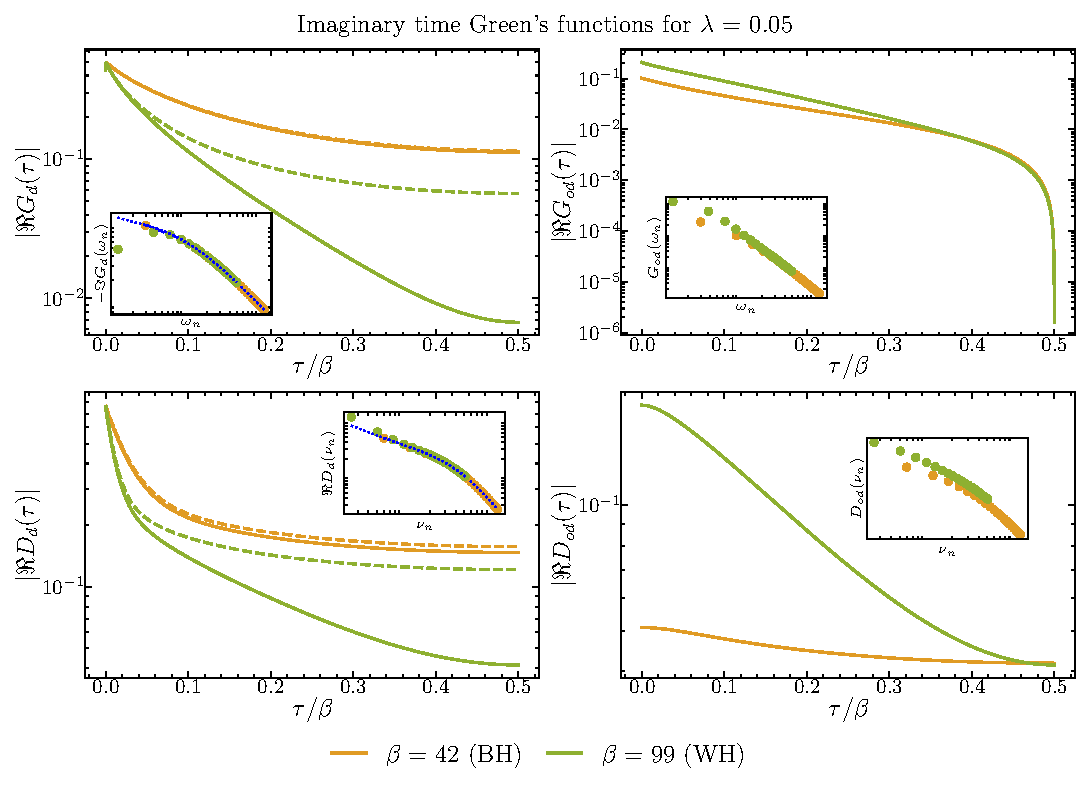
\includegraphics[width=\linewidth]{figures/chapter3/LLINSETGreenFunctionPlotsMetal.pdf}
    \caption{Imaginary time Green's functions at on lowering temperature at fixed $\lambda$ in the metallic state. The dotted lines show the exact numerical solution to the one-sided model, i.e. when $\lambda = 0$, at the corresponding temperature. These figures indicate that in the wormhole phase, off-diagonal correlations are enhanced and diagonal correlations are suppressed. The insets show the frequency dependence of the respective Green's functions.}
    \label{fig:GreenFunctionPlotsMetal}
\end{figure}


On further lowering temperature to $T\lesssim \lambda$ at low $\lambda \ll g^{2}/\omega_0^2$ the state with power law correlations changes over into a state with exponentially decaying correlations in a first order phase transition. This is shown in the green curves in Fig.~\ref{fig:GreenFunctionPlotsMetal}. This is a phase transition driven by the tunneling coupling as predicted and as can be seen by  comparison to the single sided YSYK Green's function for the same variables. The new state is the TFD/Wormhole state characterized by a gap and a linearly periodic spectrum $E = E_{\text{gap}}(1+\frac{1}{\Delta} n)$. The gap is directly visible in the single fermion Green's functions in their exponential decay at large times  
\begin{align}
    G_d(\tau) \sim e^{-\gamma \tau}. 
\end{align}
%Unlike the free-fermion state FF, for which $\gamma = \lambda$, the exponent varies as a function of $\lambda$ as is varied at a constant temperature. 
The size of the gap $\gamma$ is controlled by $\lambda$ and its leading functional dependence can be understood from the scaling properties of the tunneling interaction as a perturbation of the quantum critical state \cite{maldacena2018eternal}. In the bilocal formulation of the action this term is (see Appendix.~\ref{app:effectiveaction} Eq.\eqref{eq:Sf}) 
%\comment{CHECK}\as{done}
\begin{align}
\label{eq:tunneling-interaction}
    S_{\text{tunnel}} =\int\dd\tau\dd\tau' \lambda G_{12}(\tau,\tau')~,
\end{align}
and hence at the quantum critical point $\lambda \sim \Lambda^{2-2\Delta_f}$ where $\Lambda$ is the RG scale of the theory.
Hence just below the transition we expect the gap to scale as 
\begin{align}
    \gamma[\lambda] \sim \lambda^{\frac{1}{2-2\Delta_f}}. 
    \label{eq:gapscaling}
\end{align}
This scaling is indeed seen by extracting the gap $\gamma$ from the logarithmic derivative of the single fermion Green's function $G_d(\tau)$ in the long time regime  for various $\lambda$ at fixed $T\ll \lambda$ in the TFD/Wormhole phase: Fig. ~\ref{fig:ImagTimeScaling}. The single boson Green's function exhibits the same gap $D \sim e^{-\gamma\tau}$ as there is only one energy scale that can be constructed using $\lambda$ consistent with the dimensional analysis of Eq.~\eqref{eq:tunneling-interaction}. As can be seen from the insets in Fig.~\ref{fig:ImagTimeScaling}, although the scaling of the exponent $\gamma$ with the coupling $\lambda$ is according to Eq.~\eqref{eq:gapscaling} for both the bosons and the fermions, the numerical prefactor is different for the two cases. %\comment{Do we understand why the boson Green's function must have the same gap.}\as{done}
%The mass gap $\gamma$ is extracted from the logarithmic derivative of $G_d(\tau)$ and $D_d(\tau)$ in the long time regime where we expect the exponential decay and then fit how it changes with lambda. We observe strong agreement between the dimensional analysis result and the numerical computation.  
%


\begin{figure}[t!]
    \centering
%    \begin{subfigure}[t]{0.45\textwidth}
%        \centering
        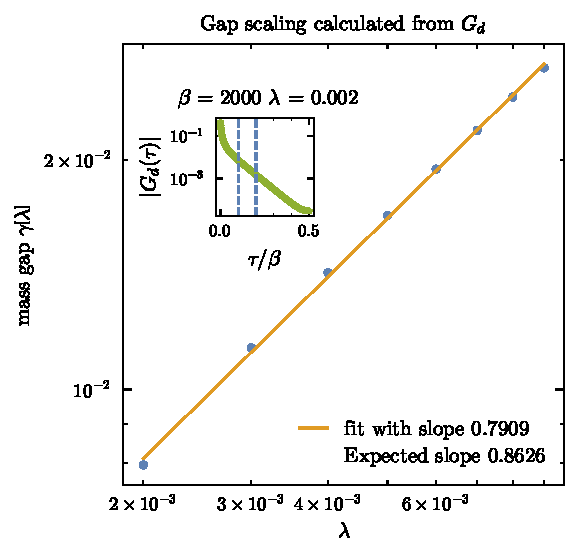
\includegraphics[width=0.47\textwidth]{figures/chapter3/GdGapscalingv2.pdf}
%        \caption{}
%        \label{fig:ImagTimeGapscalingGkappa1}
%    \end{subfigure}
%    ~\begin{subfigure}[t]{0.45\textwidth}
%        \centering
        ~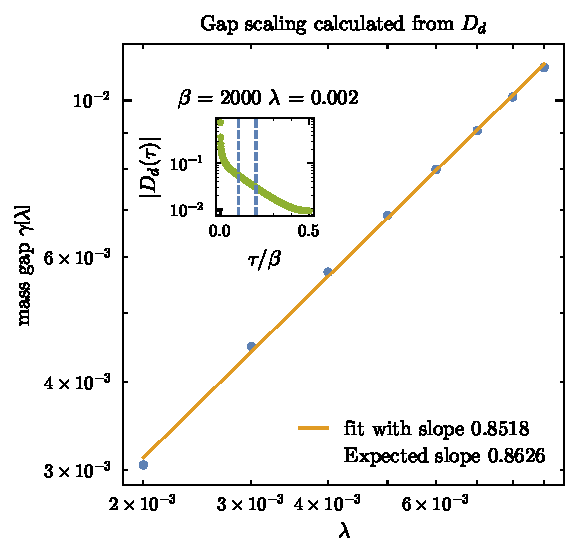
\includegraphics[width=0.47\textwidth]{figures/chapter3/DdGapscalingv2.pdf} \\
%        \caption{}
%        \label{ImagTimeGapscalingDkappa1}
%    \end{subfigure}
%    ~\begin{subfigure}[t]{0.45\textwidth}
%        \centering
        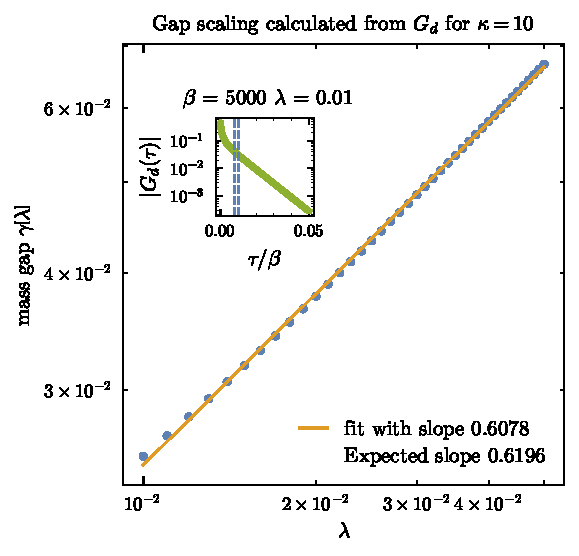
\includegraphics[width=0.47\textwidth]{figures/chapter3/kappa10GdGapscalingv2.pdf}
%        \caption{}
%        \label{fig:ImagTimeGapscalingGkappa10}
%    \end{subfigure}
%    ~\begin{subfigure}[t]{0.45\textwidth}
%        \centering
        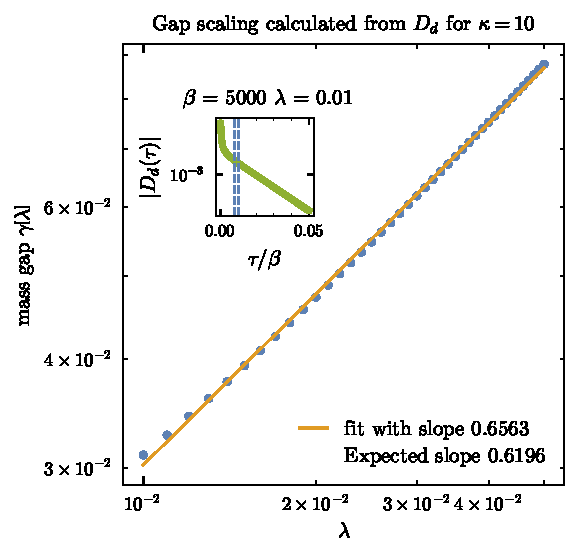
\includegraphics[width=0.47\textwidth]{figures/chapter3/kappa10DdGapscalingv2.pdf}
%        \caption{}
%        \label{ImagTimeGapscalingDkappa10}
%    \end{subfigure}
    \caption{Scaling of the gap with the cross coupling $\lambda$. Panels(a) and (b) show the diagonal fermion and boson green's function respectively for $\kappa$ = 1 and $\Delta = 0.42$ respectively. Panels (c) and (d) show the same scaling upon changing the effective slope by increasing $\kappa$ to 10, and hence reducing $\Delta$ to $0.193$. There is good agreement between the expected $\lambda^{\frac{1}{2-2\Delta}}$ scaling based on dimension analysis to the exact numerical solution. The insets show the exponential behavior of the respective Green's functions, and the window marked with the purple dotted lines indicate the region where the fit was performed for each data point of the main panels.}
    \label{fig:ImagTimeScaling}
\end{figure}
%

This specific non-analytic scaling of the gap $\gamma \sim \lambda^{\frac{1}{2-2\Delta_f}}$ with the tunneling strength is the first indication that the gapped state obtained after the phase transition  is indeed the TFD state holographically dual to an 
%On the gravitational side, this state with exponentially decaying correlations that scale in the manner of Eq.~\eqref{eq:gapscaling} represent 
an eternal traversable wormhole(WH) geometry. The more detailed prediction is that the spectrum also has linearly spaced excited states. This would be very clearly visible as peaks in the frequency spectrum in numerical solution to the real time Schwinger-Dyson equations. Though in the real time numerics in 
Fig.~\ref{fig:GreenFunctionPlotsMetalv2} we can clearly see the gap development  in the emergence of a single peak as temperature is lowered from $T\gg \lambda $ to $T\ll \lambda$, no other peaks are visible for the parameters and accuracy with which we are able to solve the system. This is in contrast to the results for Majorana and complex-SYK in \cite{pluggeRevivalDynamicsTraversable2020a,sahoo_traversable_2020}
 where these excited states are clearly visible in the spectral density $\rho \sim -\text{Im}G$. 
However, we are able to see signatures of precisely these linearly spaced excited states in the numerical solution to the imaginary time Schwinger-Dyson equations. The imaginary times numerics are more stable and we are able to compute at much lower temperatures where thermal broadening plays less of a role. For a system with well defined asymptotic states that only interact locally the asymptotic Greens function in imaginary time at very low temperature will take the form
\begin{align}
    G(\tau) \sim a_0e^{-E_0\tau} +a_1 e^{-E_1\tau} +a_2e^{-E_2\tau} +\ldots
    \label{eq:SumExponentsSchem}
\end{align}
Here $E_0, E_1, E_2, \ldots$ are the energies of the lowest excited states.
Fig.~\ref{fig:subleadingexponentGD} shows that subtracting out the dominant contribution of the gapped groundstate with $E_0 = c\Delta$ shows a clear remaining exponential decay whose exponent should be proportional to $E_1 = c(\Delta+1)$. We know the analytic value of $\Delta= 0.42037\ldots$ for these parameters, see Appendix~\ref{app:confoneside}. 
%\comment{FILL IN VALUE; SHOW/REFER TO COMPUTATION IN APPENDIX}\as{done}. 
From this we can extract $c=E_{gap}/\Delta$ and predict $E_1=c(\Delta+1)$. The predicted slope is up to two digits accurate with the fitted slope; see Fig.~\ref{fig:subleadingexponentGD}. This is a strong second sign that the state at $T\lesssim \lambda$ for $\lambda\ll g^{2}/\omega_0^2$  is indeed the TFD/wormhole state of the YSYK model.\footnote{Fitting multiple exponentials is notoriously difficult and small fitting adjustments can result in large changes in the value of the exponent. A visible cue is the residuals after the leading exponential(s) is/are subtracted. The remainder needs to extend at least for a small window into the previously fit region with no kink at the edge of the fitting region, as a sign that the data was not overfit.}
 

\begin{figure}[!t]
    \centering
    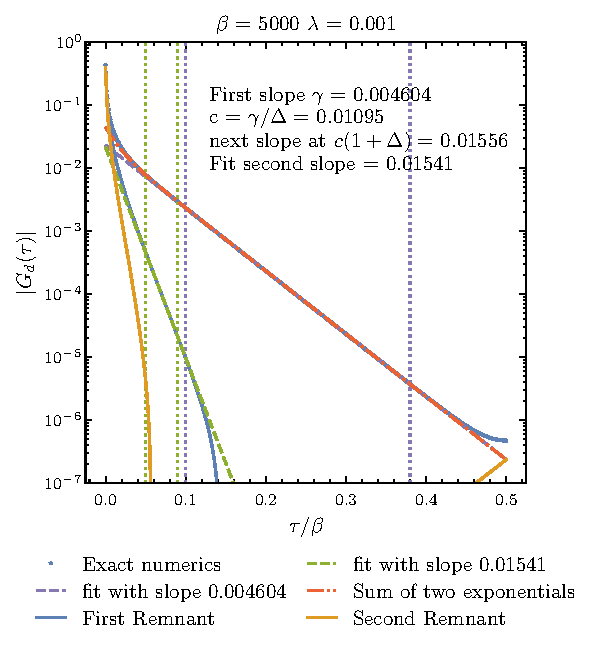
\includegraphics[width=0.75\linewidth]{figures/chapter3/ExponentsGD.pdf}%figsize actually one column
    \caption{First subleading exponent in the imaginary time numerics. The vertical dotted lines of each color indicate the window at which the fit of the corresponding color was performed.}
    \label{fig:subleadingexponentGD}
\end{figure}

\begin{figure}[!t]
    \centering
    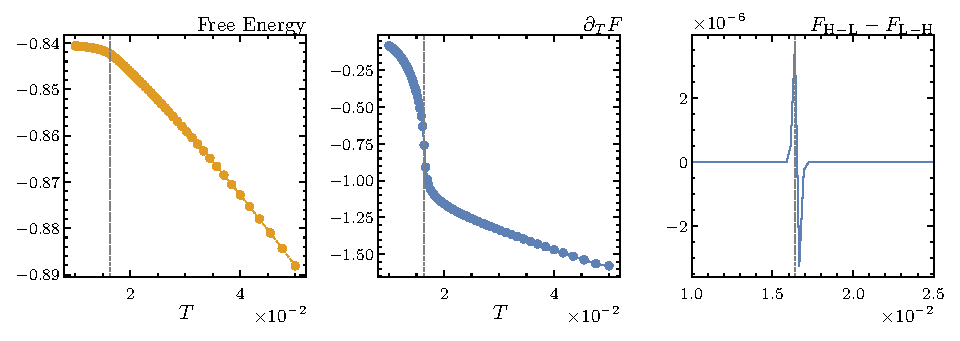
\includegraphics[width=0.95\linewidth]{figures/chapter3/ButterFlyPlot.pdf}
    % 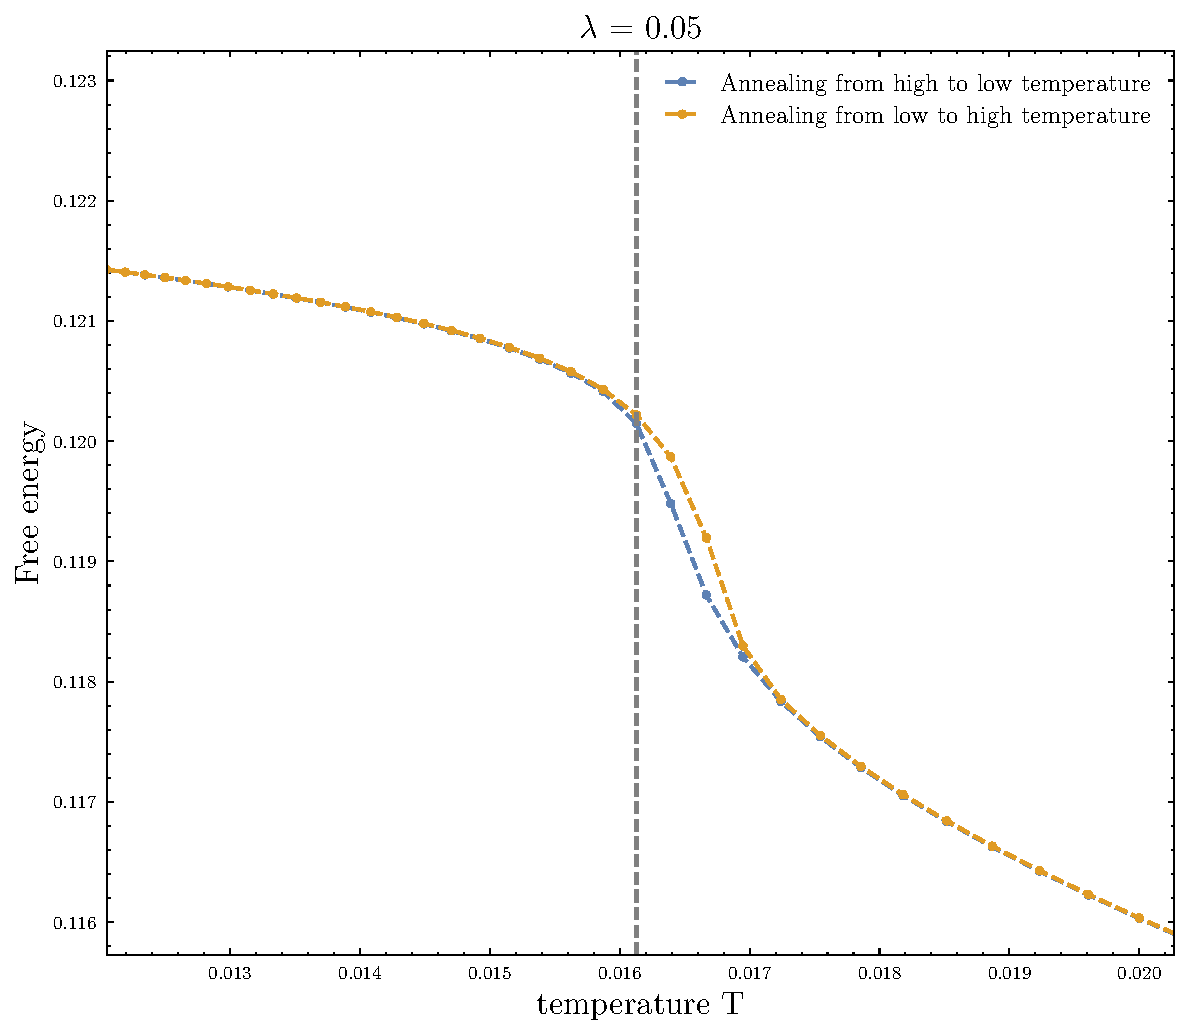
\includegraphics[width=0.9\linewidth]{butterflyplotmetal.pdf}
    \caption{Free energy as a function of temperature for $\lambda = 0.05$. The dashed gray line represents an estimate of the wormhole transition temperature, when the Green's functions cross over from power law to exponential decay. For this value of $\lambda$, our numerical solution was unique at every chosen value of the temperature, save a couple of instances close to the transition, where it shows mild hysteresis. This is delineated in the right panel which shows the difference in free energy between the solutions obtained from annealing from high to low temperature ($F_{H-L}$), and low to high temperature ($F_{L-H}$), by using as an initial guess at each step the solution obtained at the previous step.
    % \comment{THERE IS SOMETHING WRONG IN THE FIGURE. THE UPPER CURVE SHOULD BE THE ANNEALING FROM HIGH T TO LOW. AND THE LOWER CURVE SHOULD BE THE CURVE FROM LOW TO HIGH. PLEASE CHECK}
    }
    \label{fig:butterflyplotmetal}
\end{figure}

%\as{written short passage on phase transition}
In  coupled Majorana \cite{maldacena2018eternal,pluggeRevivalDynamicsTraversable2020a} and complex SYK models \cite{sahoo_traversable_2020} the physics underlying the diagonal Green's functions jump from power law to exponential decay is a first order phase transition. In the gravitational dual this is a so-called Hawking-Page transition between a two black hole configuration and a wormhole.
%\comment{CHECK THAT IT IS A PHASE TRANSITION BETWEEN A TWO SIDED BH AND NOT TWO BHs}.
%
%For values of $\lambda$ not too small, we see a distinct first order phase transition, analogously to the Hawking-Page transition, upon starting from high temperature and successively annealing to lower temperatures at a scale $T \sim \lambda$. At this temperature the diagonal Green's functions jump from power law to exponential decay. 
As the gravitational dual of quantum critical ground state of the non-superconducting Yukawa-SYK and Majorana and complex SYK models are essentially the same, we expect the same here. This is what we find and is illustrated in the free energy of the coupled YSYK system shown in  Fig.~\ref{fig:butterflyplotmetal}. 
Though not perfectly discontinuous, the derivative of the free energy exhibits a clear jump. Furthermore, while for temperatures away from the critical point, the numerical solution is unique upon annealing both upward and downward in temperature, there is a hysteresis near the phase transition indicating that it is indeed first order. The hysteresis is small and not as sharp as in simpler models, but it is clearly there. 
It is supported by our observation that in our numerics
%Numerically, we  see that 
the iterations take longer and longer to reach the convergence threshold for temperatures very close to the transition, as the system struggles to find the true ground state.\footnote{At very low temperatures and very small $\lambda$ however, we find that the annealing in temperature is not sufficient as a numerical procedure to find the true ground state as the difference in free energy between the two distinct minima become smaller than the precision with which we can calculate our numerical solutions. 
% Annealing in $\lambda$ instead was used to overcome this.
}
%This is illustrated quite clearly in the free energy shown in  Fig.~\ref{fig:butterflyplotmetal}. 
%For temperatures away from the critical point, the numerical solution is unique upon annealing both upward and downward in temperature, but exhibits hysteresis near the phase transition.
%At very low temperatures and very small $\lambda$ however, we find that the annealing in temperature is not sufficient as a numerical procedure to find the true ground state as the difference in free energy between the two distinct minima become smaller than the precision with which we can calculate our numerical solutions.

%To overcome this, 
We note that the YSYK TFD/wormhole solution 
can also be obtained alternatively in a smooth manner by starting from the nearly free fermion thermal state FF at large $\lambda \gg g^{2}/\omega_0^2$ but low $T\ll \lambda$ described above, and then reducing $\lambda$. No phase transition is seen. Instead the gap dependence on $\lambda$ changes smoothly from $\gamma_{\lambda \gg} \sim \lambda+\ldots$ as in Fig.\ref{fig:LargeLambdaGapScaling} to $\gamma_{\lambda\ll} \sim \lambda^{\frac{1}{2-2\Delta_f}}$ exhibited in Fig.~\ref{fig:ImagTimeScaling}.
% \comment{DO WE HAVE FIGURE OF THE TRANSITION? IF NOT, THEN NOT. IT WOULD HAVE TO BE OF THE FREE ENERGY.}\as{I don't think I understand what you mean - we have Fig.~\ref{fig:LargeLambdaGapScaling} showing linear scaling at large $\lambda$ and we have Fig.~\ref{fig:ImagTimeScaling} showing the non-analytic scaling at small lambda. I don't have a figure showing the entire range, but I can try to make something if this is what you mean.}\comment{It would have been nice to show a plot of $\gamma(\lambda)$. For now, we leave it: As stated if not, then not. Comment this out once you agree.}

% \begin{figure}[h]
%     \centering
%     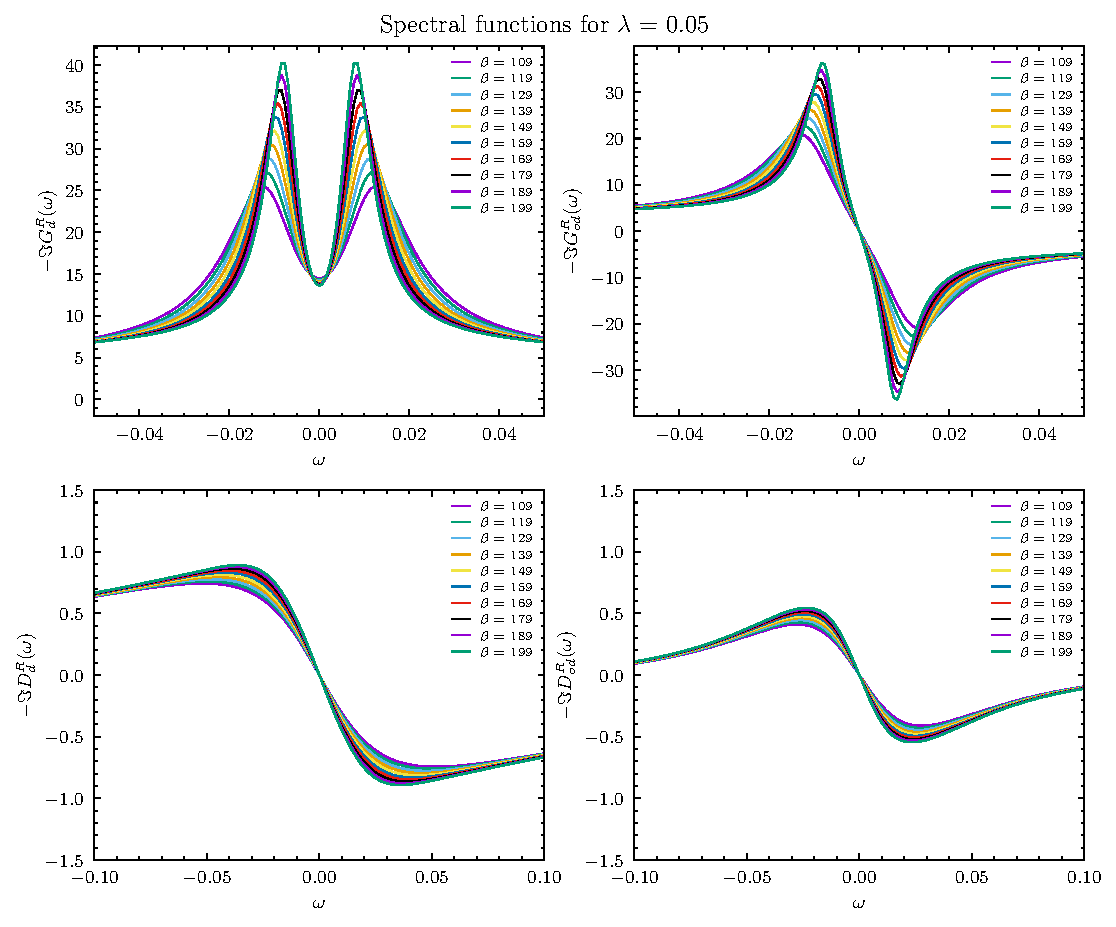
\includegraphics[width=\linewidth]{v1TempEvolnSpectralGapMetalWH.pdf}
%     \caption{Temperature evolution of wormhole spectral function. The wormhole state is characterized by a single split peak, and the tower of conformal states is not observed in our numerics. This can be compared to the spectral function in the large $q-$ limit of study of Qi and Zhang (Ref.~\cite{qiCoupledSYKModel2020a}).}
%     \label{fig:GreenFunctionPlotsMetalv1}
% \end{figure}

\begin{figure}[t!]
    \centering
    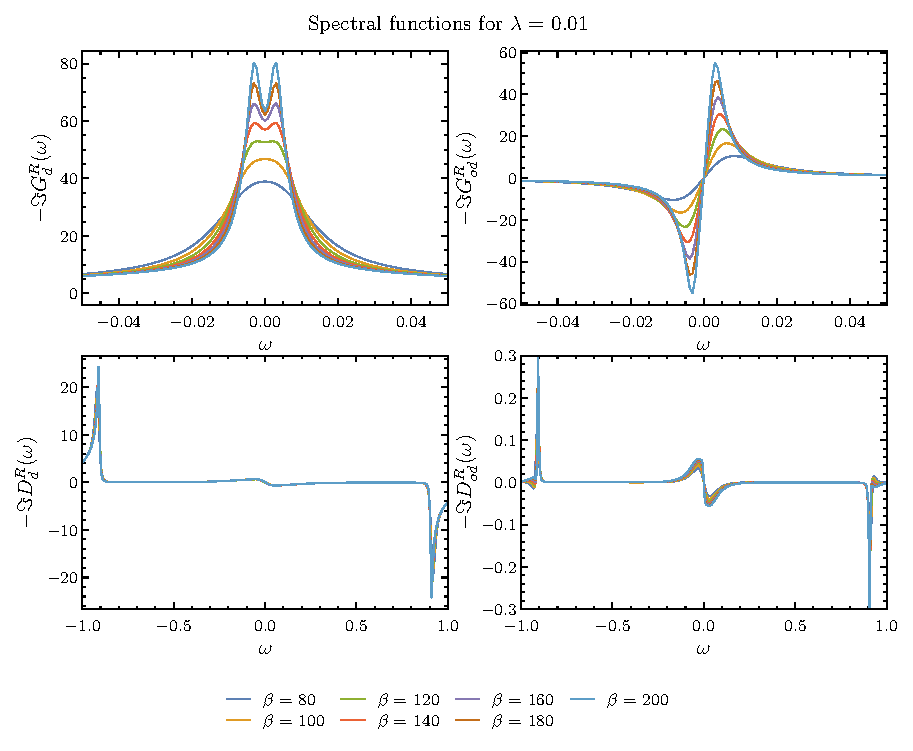
\includegraphics[width=\linewidth]{figures/chapter3/v3TempEvolnSpectralGapMetalWH.pdf}
    \caption{Temperature evolution various spectral functions in the model. The wormhole state is characterized by two symmetrically placed split peaks, but the black hole state is characterized by a smooth spectral function with the quantum critical form. 
    % This can be compared to the spectral function in the large $q$- limit of study of Qi and Zhang (Ref.~\cite{qiCoupledSYKModel2020a}).
    }
    \label{fig:GreenFunctionPlotsMetalv2}
\end{figure}



%#
%\newpage
\section{Inclusion of superconductivity: the BCS Josephson wormhole}
\label{sec:sc-state}

We now probe whether this YSYK TFD/wormhole state survives the inclusion of superconductivity. To do so we turn on the possibility of a non-vanishing pair-condensate $\langle F\rangle\neq 0$ by setting $\alpha=0$.
For simplicity we shall first look at the specific model where the phase of $\lambda=|\lambda|e^{i\theta}$ is set to vanish: $\theta=0$. In this case, both sides are identical to one another --- there is an explicit mirror symmetry $c_1 \leftrightarrow c_2$ and the superconducting state will also be mirror symmetric under this symmetry.
In a spatially extended system, this would correspond to the situation where the phases of the superconducting condensates in both of the subsystems are by construction aligned.
 
\begin{figure}[t!]
    \centering
    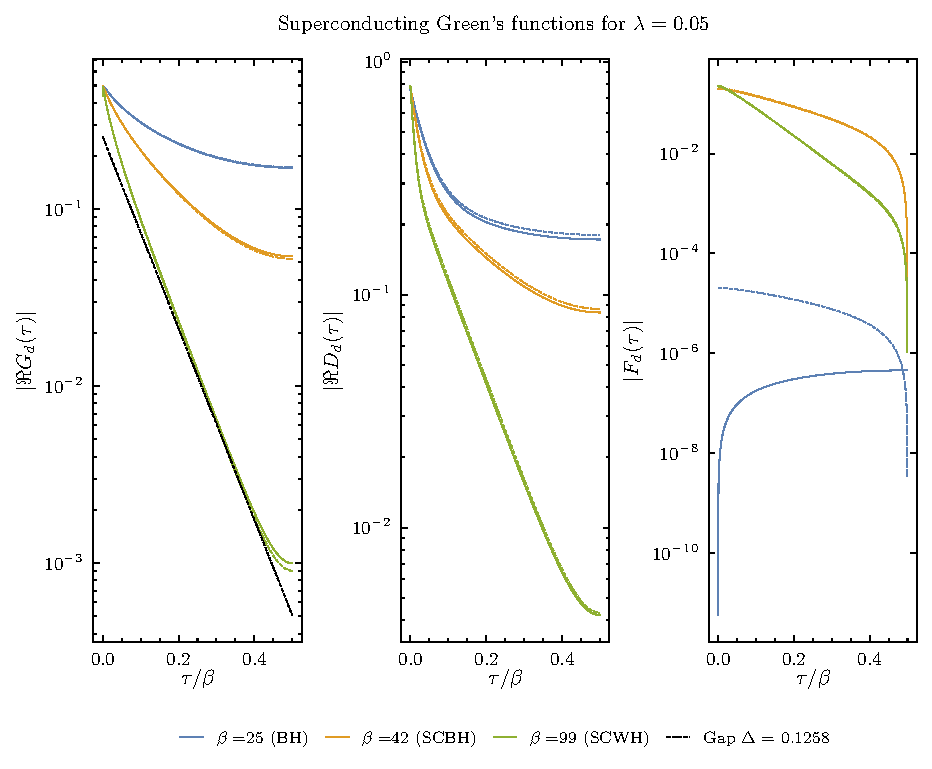
\includegraphics[width=\linewidth]{figures/chapter3/SupCondFigs.pdf}
    \caption{Superconducting solutions to the two sided model. The solid lines show the full solution to the two sided model, and the dashed line shows the numerical solution to the one sided model. The two are almost identical to one another.}
    \label{fig:SuperconductingGFsImagTime}
\end{figure}

Fig.~\ref{fig:SuperconductingGFsImagTime} shows the exact numerical solution to the saddle point equations now including the presence of the anomalous propagator terms $F_d$ and $F_{od}$. 
For the parameters we studied we know based on the time-reversal symmetry breaking $\alpha=1$ model roughly at which temperature to expect the transition to the TFD/wormhole state. 
%The temperature at which the system becomes superconducting is a priori not known. 
We have {\em specifically} chosen parameters $g/\omega_0^{3/2} =0.5$, 
%however, 
such that this descent into superconductivity happens from the thermal quantum-critical state holographically dual to a BH (see Fig.~\ref{fig:YSYK-phase-diagram}). From the single sided YSYK model we also know that for these parameters this superconducting transition temperature is higher than the TFD/wormhole transition temperature: $T_c > T_{TFD}$.
%\comment{CHECK}\as{correct}\comment{CAN WE SHOW THIS IN A FIGURE, FIRST CHECK BELOW, MAYBE WE DO THIS ALREADY) } \as{Yes, we show this both in the free energy figure, and also in the temperature dependence of the critical current figures below. Please remove if agreed.}
The question therefore is whether {\em after} the transition to superconductivity there is still a transition/crossover to a TFD/wormhole like state as one lowers the temperature further.


The numerics indicate that this is so, but the identification is tenuous. 
The issue is that the superconducting state is also characterized by a gap in the single fermion spectral function $G_d$. So is the wormhole state, as we have shown.
In neither case is this the single defining characteristic, but 
%let us first 
we can determine whether the robust spontaneous symmetry breaking gap, or the fragile remnant quantum criticality induced gap is the physics that the numerics shows.
The full Green's functions in Fig.~\ref{fig:SuperconductingGFsImagTime} show that the coupled YSYK system indeed first transitions to a superconducting state --- the appearance of a non-vanishing order parameter $\Delta = \abs{F_d(\tau=0^+)}$ %\comment{CHECK. NOT $\Delta = \int d\tau F(\tau)?$} \as{Strictly speaking, it should indeed be $F(i\omega\rightarrow 0)$, but we don't show $F(\omega)$ anywhere in this article, and for practical purposes $\abs{F(\tau=0)}$ is sufficient as a diagnostic. In my opinion it's better to say $\abs{F(\tau)}$, but I'm also happy to say $\abs{F(i\omega_1)}$.} 
in the right column. At this time the asymptotic behavior is not yet recognizable as the exponential decay corresponding to a gap. %\comment{but the real time numerics can? or what can?}\as{Real time spectral function can, but we don't have it now.}\comment{OK, then we leave it for now. Comment out if you read this.} 
This is so, because for the value $g/\omega_0^{3/2}=0.5$ the gap develops BCS-like by opening up and is very weak for $T\lesssim T_c$ \cite{esterlis2019cooper}. For $T \ll T_c$ one does clearly see a gap in the green curve in Fig.~\ref{fig:SuperconductingGFsImagTime}. This is also the regime where one would expect the TFD/wormhole gap to arise.
The gap that is present is the ordinary BCS superconducting gap, however. This follows from a direct comparison with the result for a single sided YSYK  model at the same parameters, but absent tunneling ($\lambda=0$). Fig.~\ref{fig:SuperconductingGFsImagTime} 
%\comment{THE REFERENCE SHOULD BE FIG.\ref{fig:SuperconductingGFsImagTime}, RIGHT?}\as{yes that's a typo - I've changed it now}
%\comment{TO ADD}\as{added - the fit to the boson is not so good, but the fermion one is very good} 
shows that the dominant exponential scaling is the same. 
\begin{figure}[t]
    \centering
    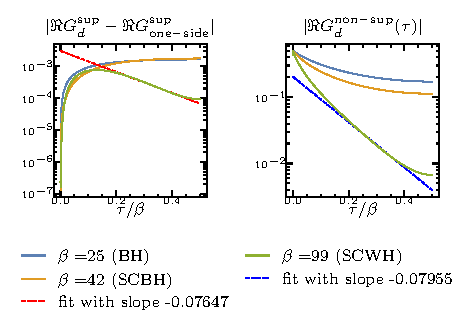
\includegraphics[width=\linewidth]{figures/chapter3/diffG.pdf} %figsize is actually one column
    % ~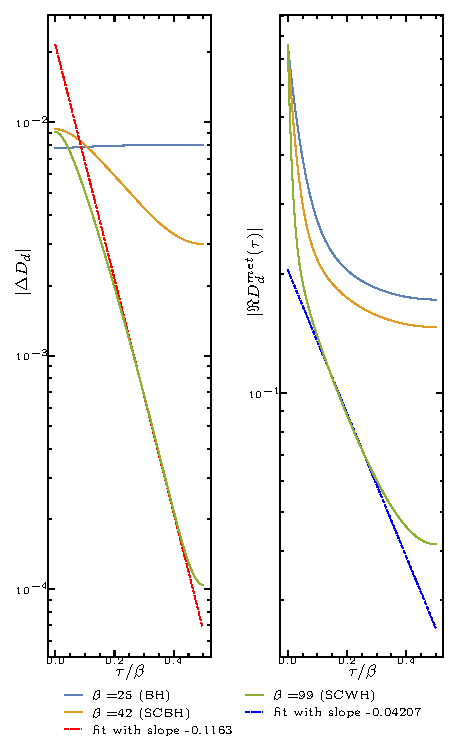
\includegraphics[width=0.45\linewidth]{diffD.pdf}
    \caption{A remnant of the wormhole can be seen if one subtracts the one sided Green's functions from the diagonal Green's functions of the two sided tunneling coupled model.}
    \label{fig:subleading-Sc}
\end{figure}

\begin{figure}
    \centering
    % 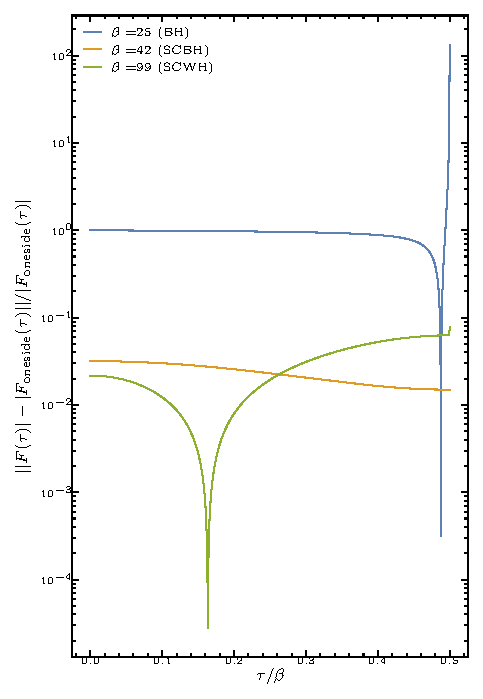
\includegraphics[width=0.5\linewidth]{ratioFs.pdf}
    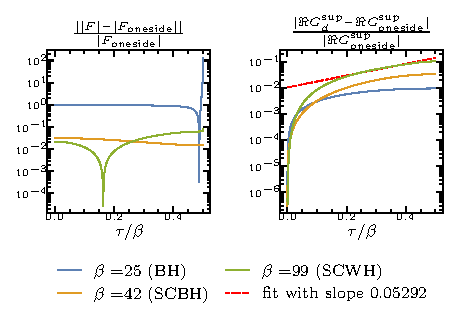
\includegraphics[width=0.9\linewidth]{figures/chapter3/ratioFsv2.pdf} %figsize is actually one column
    \caption{The anomalous propagators mostly just follow the one sided anomalous propagators, except for a small shift in magnitude. In the green curve, one sees a dip because the difference changes sign, and the absolute value is plotted on a log scale. The shift in magnitude is to be expected because in one case $\lambda \neq 0$, and this changes the magnitude of the solutions, but does not change the qualitative form.}
    \label{fig:Fratio}
\end{figure}
The indication that this is nevertheless also a TFD/wormhole state follows removing the contribution of the superconducting component. Taking the difference of the coupled YSYK model with the single-sided YSYK model with no tunneling shows that a distinct subleading exponential form remains in the single fermion response $G_d$ of the coupled model; see Fig.~\ref{fig:subleading-Sc}.
%\comment{HERE SHOULD BE THE REFERENCE TO FIG.\ref{fig:subleading-Sc}, RIGHT?} \as{yes}. 
%In the anomalous Green's function $F_d(\tau)$ the subtraction of the single sided response leaves a remnant that simply follows $F(\tau)$ of the one sided model but with a much smaller magnitude - this just means that its magnitude is shifted by a small constant, but with the function containing no additional structure. We also observe that the off-diagonal terms of the anomalous propagator $F_{od}(\tau)$ are numerically vanishingly small. The condensate sector is therefore completely equivalent between the single sided YSYK model and the tunneling coupled model, i.e. the condensing Cooper pairs are well formed separately on either side, and there is no cross-condensation or cross-excitation tunneling. In particular this means there are no (observable) excited states in the pairing channel, or any indication of tunneling physics. 
%
%\as{This paragraph needs editing still} At the same time, 
This residual exponential in the single fermion response can be compared with the leading exponential of the TFD/wormhole state in the absence of superconductivity. The exponent of the remnant exponential decay in the superconducting state is within $10\%$ of that of the TFD/wormhole value. 
% A small change due to level repulsion from the changed value of the gap is expected, but the equivalence of the condensate to the uncoupled state and no pairing excitations together with this near equivalence strongly suggests that the presence of superconductivity has solely rearranged the groundstate of the system and has left the excitations mostly unchanged. 
We can understand this through a simple Landau-Tisza two-fluid model. A fraction of fermions on the superconducting sector form pairs and enter the condensate. The other fermionic sector parallels the $\alpha=1$ non superconducting TFD/wormhole state discussed in Sec.~\ref{sec:metallic-state}, and also holds some spectral weight, as is illustrated in Fig.~\ref{fig:subleading-Sc}.

Numerical accuracy prevents us from testing more firmly whether the superconducting state below $T<T_{\text{WH}}$ is indeed a TFD/wormhole state built on a BCS-groundstate with higher excited states which should also follow the wormhole pattern. Our knowledge of ordinary BCS superconductors, however, supports that this only slightly changed first excited state can be taken as a convincing signature of the equivalent state of the TFD/wormhole state in the non-superconducting model. 
% In ordinary BCS superconductors with s-wave pairing, cooper pairs all condense to the same quantum state as soon as they form. Fermionic excitations to the system can be created by breaking of the Cooper pairs, which cost binding energy $\Delta$.
% In BCS superconductors the temperature at which electrons form a bound Cooper pairs is lower than the naive condensation temperature at which the bosonic Cooper pairs condense.
% \as{The previous sentence doesn't make sense to me. I would say something more like - In BCS theory, the ground state is formed by a coherent state of cooper pairs. Excited states are formed by the breaking of cooper pairs, which cost binding energy $\Delta$.}\comment{I kept the text but added yours. Please check}\as{I still don't understand what it means.}
% The corollary of this statement is that although the ground state is formed by a coherent state of Cooper pairs, excited states are formed by the breaking of Cooper pairs, which cost binding energy $\Delta$. 



The excitation spectrum above the BCS-groundstate does not contain any finite energy Cooper pair 
excitations. 
All low energy excitations are based on the (dressed, gapped) fermionic excitations in the theory. The TFD state of a BCS-like superconductor will therefore formally be very similar to the TFD state of a gapped fermion system without superconductivity.\footnote{Of course in a real superconductor this simplified picture does not hold completely. There are order parameter fluctuations supported by gradients. Such order parameter fluctuations can always be excited at finite temperature. Correspondingly a TFD state for these should exist. The SYK model is a quantum dot and there are no spatial gradients that can support a finite phase space of order parameter fluctuations. The simplified notion therefore does work here.} 
% \comment{ADDED FOOTNOTE. CHECK}
% This is indeed what our numerics shows, in that the subleading exponential in the single fermion Green's function of the coupled superconducting YSYK model are small perturbations of the non-superconducting YSYK model. 
This is indeed what our numerics shows, in that the single fermion Green's function of the coupled superconducting YSYK model are the made up of a weighted sum of the one-sided superconducting model and the two-sided non-superconducting YSYK model. 

It is further supported by studying the anomalous Green's function $F_d(\tau)$. Here the subtraction of the single sided response leaves a remnant that simply follows $F(\tau)$ of the one sided model but with a much smaller magnitude - this just means that its magnitude is shifted by a small constant, but with the function containing no additional structure. We also observe that the off-diagonal terms of the anomalous propagator $F_{od}(\tau)$ are numerically vanishingly small. The condensate sector is therefore completely equivalent between the single sided YSYK model and the tunneling coupled model, i.e. the condensing Cooper pairs are well formed separately on either side, and there is no cross-condensation or cross-excitation tunneling. In particular this means there are no (observable) excited states in the pairing channel, or any indication of pair-tunneling physics. 


From the gravitational perspective it is perhaps surprising that certain excitations --- single fermion --- can traverse the wormhole and others --- Cooper pairs --- cannot. At this stage we have only shown the single fermion response function, and not the Cooper pair response function. This would correspond to a four-point function in terms of elementary fermionic excitations. In the large $N$ limit in which we compute and which is the limit in which a dual gravitational description emerges, such a four-point function is suppressed at order $1/N$. Formally at the order we work there are no correlations whatsoever between Cooper pairs. This absence of correlations thus matches the microscopic YSYK perspective. At the same time it also indicates that a true answer whether the wormhole supports Cooper pair tunneling and revivals requires this four-point function computation. We leave this for future work.

From this microscopic viewpoint one would also expect Cooper pair tunneling and a Cooper pair TFD/wormhole state in a BEC like superconducting state where Cooper pairs can exist as uncondensed excitations. This regime exists in YSYK models for larger $g/\omega_0^{3/2} \sim 1$ identifiable by the fact that the superconducting gap fills as $T$ increases, rather than closes \cite{esterlis2019cooper}. The issue is that in this regime the metallic state is not the quantum critical groundstate gravitationally to a two-sided black hole. As revivals can arise for many different reasons and it is precisely the  level spacing in the spectrum inherited from the quantum critical state that we use to identify the wormhole, it is not clear how we could identify a BEC-like superconducting TFD/wormhole.

%
%


%\comment{I do not understand below}\as{edited}
At very large $\lambda$, we do not find any evidence of superconductivity, even down to the lowest temperatures that we can reach in our numerics. This can be understood because the metallic state in this case is a conventional gapped free fermion state at charge neutrality. There is no macroscopic density of states at zero energy; there is no density at all. There is no reservoir for Cooper pairs to form or condense.
%with the fermions forming a singlet across the two sides. The fermion diagonal spectral functions is the simply gapped with a delta peak at a large $\lambda$, and it is not surprising that this trivial state is unable to be induced to superconduct at low temperatures.
%
%This evidence that the phase of the superconducting wave function is well defined on either side is indication that the phase may be twisted independently giving rise to a Josephson-like effect. 
%\comment{EDITED.PLEASE CHECK} \as{checked - fixed minor typos}
\newcommand{\eps}{\epsilon}
\section{A standard Josephson current}

This observation that the TFD/wormhole state of the coupled model is built on a direct-product groundstate of two essentially independent condensates with no observable overlap suggests that its Josephson physics is standard. This is indeed the case. It is a well known trick in the conventional BCS Bogoliubov-deGennes formulation of Josephson physics that the external phase difference can be moved to the phase of the tunneling coupling $\lambda$ (see e.g. \cite{tummuru2022josephson}). 
This follows from the fact that a change of variables $c_2\rightarrow c_2e^{i\theta}$ can be compensated by a change in $\lambda \rightarrow \lambda e^{-i\theta}$. Thanks to the earlier mentioned mirror symmetry, this remains a solution to the saddle point equations, this change of variables will simply change the phase of the saddle-point solution of the second anomalous Green's function $F_{22}\rightarrow F_{22}e^{2i\theta}$ w.r.t. to the first anomalous Green's function.  If the two superconductors are connected by a (metallic) ring-like configuration as well $\theta$ equals the magnetic flux through the loop in units of the superconducting flux quantum $\frac{h}{2e}$ (set to unity in our conventions). A sudden quench of $\lambda e^{i\theta} \rightarrow \lambda$ then sets up a configuration where the BCS condensate in the second system differs by a phase, but this is no longer the exact groundstate. The relaxation to the groundstate is the Josephson current. 
%If the two superconductors are connected by a (metallic) ring-like configuration as well $\theta$ equals the magnetic flux through the loop in units of the superconducting flux quantum $\frac{h}{2e}$.
%\comment{CHECK. IS THIS INTERPRETATION CORRECT}\as{yes}

The one difference between the YSYK model and the conventional BCS system is that the mean-field kinetic part of the action also has non-neglible contributions to the off-diagonal Green's functions. This is due to the strong coupling nature of the theory at low energies. These off-diagonal Green's functions must all be directly proportional to the tunneling coupling $\lambda$: They vanish when $\lambda=0$. In the protocol to set up the Josephson configuration, these off-diagonal Green's functions must therefore instantaneously follow the quench that rotates the tunneling coupling.
To clarify what we point out, recall that the Josephson Hamiltonian for two coupled conventional mean-field BCS system whose free energy gives the Josephson current is
\begin{align}
    H_{\text{BCS-BdG-Josephson}}(k) &= \begin{pmatrix} c^{\dagger}_{1\uparrow} & c_{1\downarrow} & c^{\dagger}_{2\uparrow} & c_{2\downarrow} \end{pmatrix}\left(
    \begin{array}{cccc}
     \eps(k)  & \Phi  & \lambda & 0 \\
     \Phi  & -\eps(k)  & 0 & -\lambda \\
     \lambda^{\dagger} & 0 & \eps(k)  & \Phi  e^{-2 i \theta } \\
     0 & -\lambda^{\dagger} & {\Phi}  e^{2 i \theta } & -\eps(k) \\
    \end{array}
    \right) \begin{pmatrix} c_{1\uparrow} \\ c^{\dagger}_{1\downarrow} \\ c_{2\uparrow} \\ c^{\dagger}_{2\downarrow} \end{pmatrix}~.
\end{align}
The Josephson configuration for the coupled YSYK system has for the kinetic part of the action following the insight that all off-diagonal Green's functions are slaved to the quench in $\lambda e^{i\theta}\rightarrow \lambda$.
\begin{align}
    S_f = -\ln\det
    \left(
    \begin{array}{cccc}
     i \omega _n -\Sigma _d  & -\Phi _d & -\lambda - \Sigma _{\text{od}} & -\Phi _{\text{od}} \\
     -\bar{\Phi} _{\text{d}} & i \omega_n -\tilde{\Sigma} _{\text{d}}  & - \bar{\Phi} _{\text{od}} & \lambda -\tilde{\Sigma} _{\text{od}} \\
     -\lambda - \Sigma _{\text{od}} & - \Phi _{\text{od}} & i \omega_n-\Sigma _d  & -e^{2 i \theta } \Phi _d \\
     -\bar{\Phi} _{\text{od}} & \lambda - \tilde{\Sigma} _{\text{od}} & -e^{-2 i \theta } \bar{\Phi} _{\text{d}} & i \omega_n -\tilde{\Sigma} _{\text{d}} \\
    \end{array}
    \right)
    \label{eq:Josephson-YSYK-action-kinectic}
\end{align}
% That this is the correct viewpoint is supported by the observation that not quenching the phase of $\Sigma_{od}$ would result in a fractional $4\pi$-periodic Josephson effect. Such an effect should only occur in a topological insulator, which YSYK is not.




%The Schwinger-Dyson equations then reveal


\begin{figure}[t!]
    \centering
    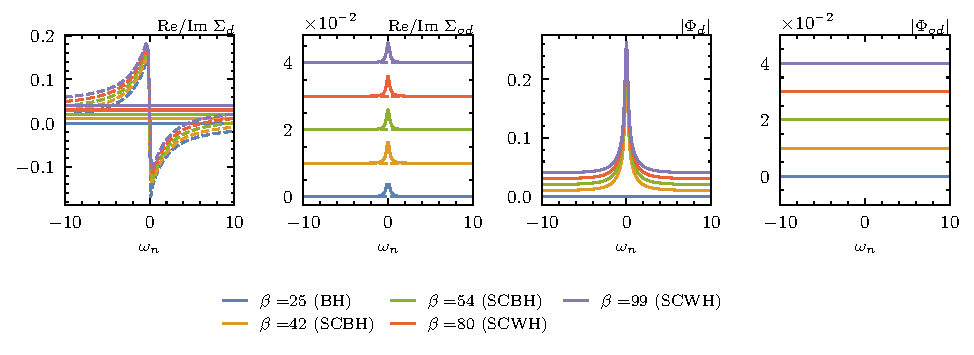
\includegraphics[width=\linewidth]{figures/chapter3/MagnitudeSEs.pdf}
    \caption{Magnitude of the various self energies in the superconducting state. In the first two panels, the solid lines indicate the real parts and the dotted lines indicate the imaginary parts. The different curves have been manually offset on the y-axis by $0.01$ each, for ease of presentation.}
    \label{fig:MagnitudeSelfEnergies}
\end{figure}


%\subsection{Josephson wormhole}

\begin{figure}[t!]
    \centering
    \raisebox{0.1 in}{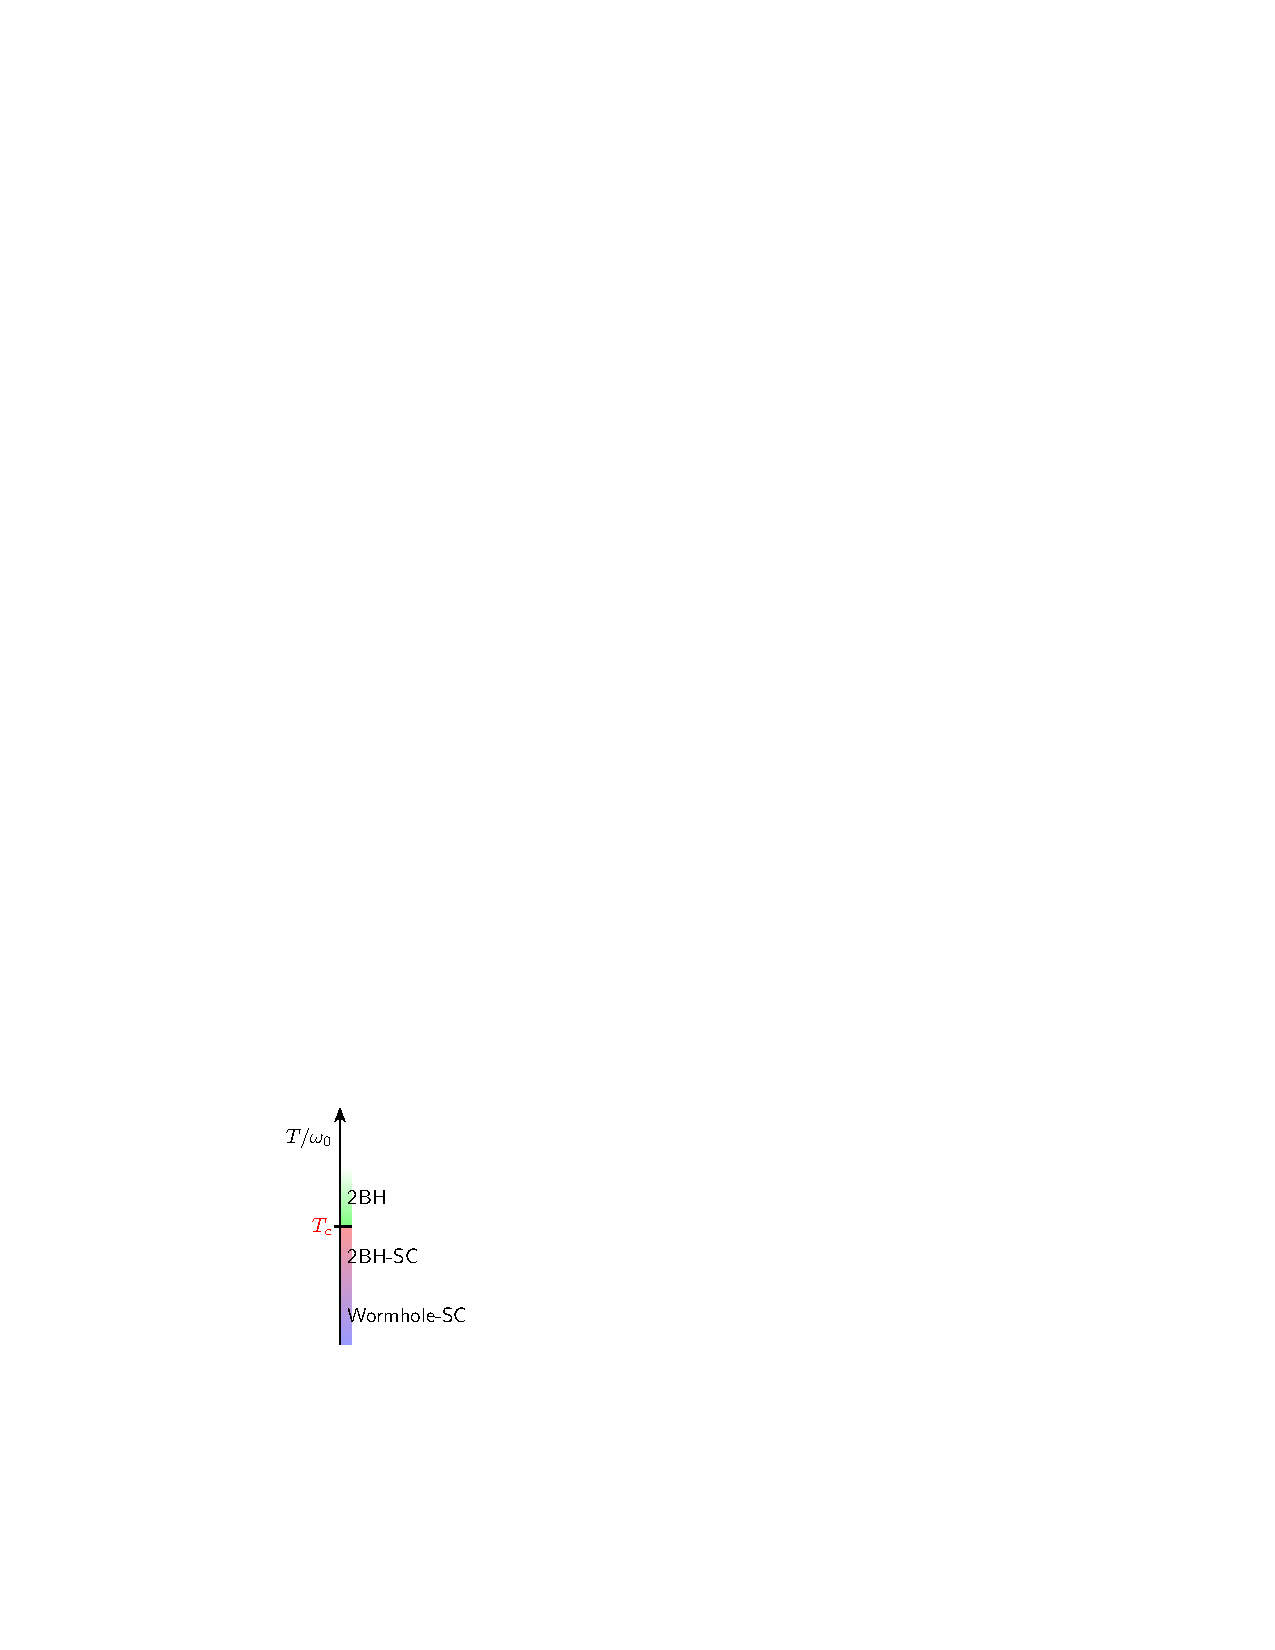
\includegraphics[width=0.2\textwidth]{figures/chapter3/SC-YSYK-PhaseDiagram-v2.pdf}}
    ~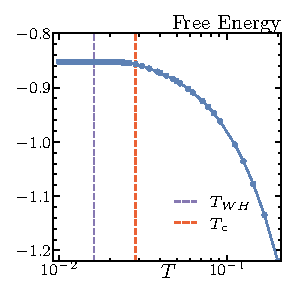
\includegraphics[width=0.35\textwidth]{figures/chapter3/SUP_free_energy.pdf}
    ~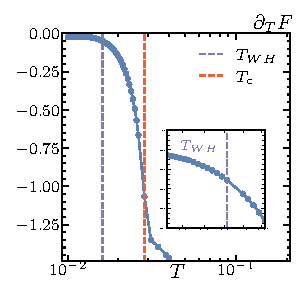
\includegraphics[width=0.35\textwidth]{figures/chapter3/partialTFSUP.pdf}
    \caption{The schematic phase diagram of the coupled superconducting Yukawa-SYK system for $g/\omega_0^{3/2}=0.5$ and $\alpha=0$. The system first transitions to from the strongly coupled finite temperature critical state (2BH) to a superconducting state (2BH-SC) in a second order transition. While superconducting the system 
    crosses over at an even lower $T$ to a superconducting TFD/wormhole state. It is no longer a first order transition.  The right shows that the free energy  has a continuous derivative at the putative transition temperature $T_{\text{WH}}$ - the inset is a zoom-in of the main panel near $T_{\text{WH}}$. 
    %The wormhole is a subleading effect; we can only establish it through the remnant exponential in the fermion green function after subtracting the one-sided part.
    }
    \label{fig:FreeEnergySupCondState}
\end{figure}

%In the double sided Yukawa SYK model, we can add a phase to the coupling term $\lambda$ and transfer the phase to the $c_2$ operator in analogy with Eq.~\eqref{eq:transphasetocops}. The theory then in terms of the new operators $c_1$ and $\tilde{c}_2$ is identical to the mirror symmetric superconducting state discussed in Sec.~\ref{sec:sc-state}. 
%
%However, in terms of the physical $c_1$ and $c_2$, the action can be written as 
% \begin{align}
%     S_f = -\ln\det
%     \left(
%     \begin{array}{cccc}
%      i \omega _n -\Sigma _d  & -\Phi _d & -\lambda -e^{-i \theta } \Sigma _{\text{od}} & -e^{i \theta } \Phi _{\text{od}} \\
%      -\bar{\Phi} _{\text{d}} & i \omega_n -\tilde{\Sigma} _{\text{d}}  & -e^{-i \theta } \bar{\Phi} _{\text{od}} & \lambda -e^{i \theta } \tilde{\Sigma} _{\text{od}} \\
%      -\lambda -e^{i \theta } \Sigma _{\text{od}} & -e^{i \theta } \Phi _{\text{od}} & i \omega_n-\Sigma _d  & -e^{2 i \theta } \Phi _d \\
%      -e^{-i \theta } \bar{\Phi} _{\text{od}} & \lambda -e^{-i \theta } \tilde{\Sigma} _{\text{od}} & -e^{-2 i \theta } \bar{\Phi} _{\text{d}} & i \omega_n -\tilde{\Sigma} _{\text{d}} \\
%     \end{array}
%     \right)
% \end{align}
% \begin{align}
%     S_f = -\ln\det
%     \left(
%     \begin{array}{cccc}
%      i \omega _n -\Sigma _d  & -\Phi _d & -\lambda - \Sigma _{\text{od}} & - \Phi _{\text{od}} \\
%      -\bar{\Phi} _{\text{d}} & i \omega_n -\tilde{\Sigma} _{\text{d}}  & - \bar{\Phi} _{\text{od}} & \lambda - \tilde{\Sigma} _{\text{od}} \\
%      -\lambda -\Sigma _{\text{od}} & - \Phi _{\text{od}} & i \omega_n-\Sigma _d  & -e^{2 i \theta } \Phi _d \\
%      - \bar{\Phi} _{\text{od}} & \lambda -\tilde{\Sigma} _{\text{od}} & -e^{-2 i \theta } \bar{\Phi} _{\text{d}} & i \omega_n -\tilde{\Sigma} _{\text{d}} \\
%     \end{array}
%     \right)
% \end{align}

The kinetic part of the action Eq.\eqref{eq:Josephson-YSYK-action-kinectic}
is the only term in the full two sided action that depends on the Josephson phase. The other terms are explicitly gauge invariant, as is evident from inspecting Eq.~\eqref{eq:Sbeforesiding}. The phase dependence of the free energy can therefore be written as 
% \begin{align}
%     \mathcal{F}  = -\sum_{\omega_n}\ln\left( f_0(\Sigma,\lambda,\omega_n) + f_1(\Sigma,\lambda,\omega_n) \cos\theta + f_2(\Sigma,\lambda,\omega_n)\cos{2\theta}\right) \,,
%     \label{eq:exactFEJosWH}
% \end{align}
% with 
% \begin{align}
%     f_1 &= 2 \lambda  \left(2 \Sigma _{\text{od}}\left(\left| \Phi _d\right| {}^2+\lambda ^2+\omega ^2\right)+\Sigma _{\text{od}} \left| \Sigma _{\text{od}}\right|
%    {}^2+4 i \omega_n  \Sigma _d \Sigma _{\text{od}}-2 \Sigma _d^2 \Sigma _{\text{od}}+\Sigma _{\text{od}}^3\right) \, ,\\
%    f_2 &= 2 \lambda ^2 \left(\left| \Phi _d\right| {}^2+\left| \Sigma _{\text{od}}\right| {}^2\right) \,
% \end{align}
% where we have also used that at the saddle point, $\Sigma_d$ is purely imaginary and $\Sigma_{od}$ is purely real, and have also dropped terms involving $\Phi_{od}$ as it is order of magnitudes smaller that the other self energies on the saddle point (see Fig.~\ref{fig:MagnitudeSelfEnergies}). 
% The origin of the $\cos\theta$ term can be understood already from the metallic case. Unlike conventional systems, the replica symmetry breaking in coupled SYK models leaves non-vanishing $G_{12}$. This has its origin in the identical realization of disorder on either side. 
\begin{align}
    \mathcal{F}  = -\frac{1}{\beta}\sum_{\omega_n}\ln\left( f_0(\Sigma,\lambda,\omega_n) + f_2(\Sigma,\lambda,\omega_n)\cos{2\theta} + g_2(\Sigma,\lambda,\omega_n)\sin{2\theta}\right) \,,
    \label{eq:exactFEJosWH}
\end{align}
with $f_2$ and $g_2$ just extracted from Eq.\eqref{eq:Josephson-YSYK-action-kinectic}.
\begin{align}
\begin{split}
   f_2 &= \Phi _d^\ast \Big(-\Sigma _{\text{od}} \Phi _{\text{od}} \Sigma _d^\ast+\Sigma _{\text{od}}^\ast \left(2 \Phi _d \Sigma _{\text{od}}-\Sigma _d \Phi _{\text{od}}\right)+2 \lambda ^2 \Phi _d-2 \lambda  \Phi _{\text{od}} \Re\left(\Sigma _d\right) 
    + 4 \lambda  \Phi _d \Re\left(\Sigma _{\text{od}}\right) \\
    &+ 2 i \omega  \Phi _{\text{od}} \Re\left(\Sigma _{\text{od}}\right)-2 i \omega  \Sigma _{\text{od}} \Phi _{\text{od}}\Big) \\ 
   &{} -\Phi _d \Phi _{\text{od}}^\ast \left(\Sigma _d \Sigma _{\text{od}}^\ast+\Sigma _{\text{od}} \left(\Sigma _d\right){}^*+\Phi _d \Phi _{\text{od}}^*\ast +2 \lambda  \Re\left(\Sigma _d\right)+2 i \omega  \left(\Sigma _{\text{od}}-\Re\left(\Sigma _{\text{od}}\right)\right)\right) 
    - \Phi _{\text{od}}^2 \left(\Phi_d^\ast\right)^2 \, , \nonumber
\end{split}
\end{align}
\begin{align}
\begin{split}
   g_2 &= i \left(\Phi _{\text{od}} \Phi _d{}^\ast-\Phi _d \Phi_{\text{od}}^\ast\right) \left(\Sigma _d \Sigma _{\text{od}}^\ast+\Sigma _{\text{od}} \Sigma _d^\ast+\Phi _d \Phi _{\text{od}}^\ast+\Phi _{\text{od}} \Phi _d^\ast + 2 \lambda  \Re\left(\Sigma _d\right)-2 \omega  \Im(\Sigma _{\text{od}})\right) \, . \nonumber
\end{split}
\end{align}
The term $g_2$ in the free energy is perhaps not familiar. However, it is generic if time-reversal symmetry is broken ~\cite{golubov2004current}. Our model preserves time-reversal, and explicit substitution shows that it vanishes 
as $\Phi_{od}=0$ (Fig.~\ref{fig:MagnitudeSelfEnergies}. There is a tiny value of order $10^{-7}$ for $\Phi_{od}(0)$ which is numerical noise.)
%\comment{Im($\phi_{od}\phi_d\star$=0?}\as{yes correct - even more simply, $\Phi_{od}=0$.}
% \comment{In the Fig.11, $\Phi_{od} \sim 10^{-7}$. Is there reason to believe this is numerical error. What would that readon be?}\as{$\Phi_{od}$ has the same units as $\lambda, \Sigma_{od}(i\omega_n)$ etc, and is just several orders of magnitude smaller. I can't think of any other reason that there can be such a huge hierarchy of scales, other than if it were actually zero, and we're seeing numerical noise. Put in another way, all these self energies are generated by the same scales in the UV : $g^{2/3}, \omega_0,\lambda$, and there's no reason why only one of them should just happen to be 5 orders of magnitude smaller than the others- which are all, expectedly, at the same scale. I still hold that it is actually zero, but  even if it weren't then it's so small that it shouldn't matter. }
% \comment{OK, can you replot it with $\Phi_{od}$ on the same scale as the others}

We can further simplify $f_2$ by observing in Fig.~\ref{fig:MagnitudeSelfEnergies} that the off diagonal self energy for the pairing $\Phi_{od}$ is vanishingly small (numerically several orders of magnitude smaller than the others). In that case, we can simply set $\Phi_{od} = 0 $ in Eq.~\eqref{eq:exactFEJosWH} to obtain 
\begin{align}
    \mathcal{F}  = -\frac{1}{\beta}\sum_{\omega_n}\ln\left( f_0(\Sigma,\lambda,\omega_n) + f_2(\Sigma,\lambda,\omega_n)\cos{2\theta}\right) \,,
    \label{eq:exactFEJosWH_afterphiodzero}
\end{align}
with 
\begin{align}
   f_2 &= 2 \abs{\Phi_d}^2\abs{\lambda + \Sigma_{od}}^2  \, .
\end{align}
This formula does not assume weak coupling, and enables us to obtain a non-perturbative expression for the Josephson current, and we can see that $\Sigma_{od}$ acts as a vertex correction to $\lambda$. 
Substituting in our previously calculated values for the various quantities, we can evaluate
%We have explicitly calculated 
Eq.~\eqref{eq:exactFEJosWH} and 
%used 
its derivative to calculate the Josephson current from the Josephson relation $I(\theta) = \partial_\theta {\cal F}$. The results are shown in Fig.~\ref{fig:JosephsonCurrent}.
\begin{figure}[t!]
    \centering
    % \resizebox{10cm}{!}{\includegraphics{foo.png}}
    \raisebox{0.01in}{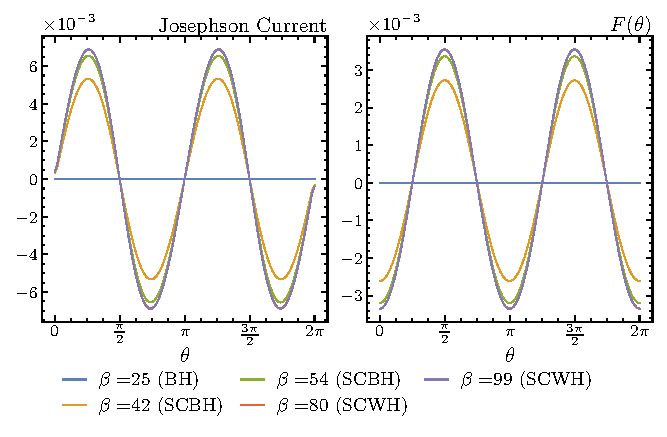
\includegraphics[width=0.6\linewidth]{figures/chapter3/JosephsonCurrent.pdf}}
   \raisebox{-0.06in}{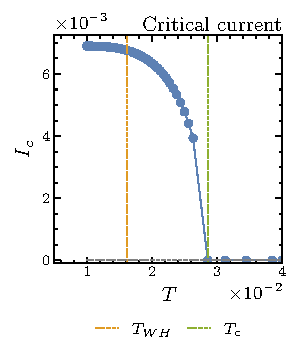
\includegraphics[width=0.34\linewidth]{figures/chapter3/TempDepCritCurrent.pdf}}
    \caption{DC Josephson current as a function of the phase angle. It should be noted that in this figure, the angle on the x-axis is the phase that was introduced on the complex hopping parameter $\lambda$, and the physical phase difference between the left and the right superconducting order parameters is $2\theta$. In the right panel, we also show the temperature dependence of the critical current, which is a measurable physical quantity.
    }
    \label{fig:JosephsonCurrent}
\end{figure}

%\as{Ref.~\cite{golubov2004current} says that the term $g_2$ in the free energy Eq.~\eqref{eq:exactFEJosWH} can only be non-vanishing if time reversal symmetry is broken. This agrees with what we have - these solutions are for $\alpha=0$. Perhaps this is the way to have solutions which have a non-zero $\Phi_{od}$, which is a necessary condition to have a nonvanishing $g_2$ - maybe this is something to look at in the future. } \comment{MOVED THIS EARLIER. PLEASE CHECK DISCUSSION THERE IMPORTANT} \as{Checked: this can be removed here.}


\section{Conclusion}
\label{sec:conclusion}

It remains remarkable that the notion of holographic duality allows in principle the study of exotic (quantum)-gravitational phenomena through ordinary strongly coupled systems. The more difficult prerequisite is that such a system must also be quantum critical. Those are not only rare, but often fragile and unstable. The most prominent instability is superconductivity. In this article, we have studied the coupled quantum critical Yukawa SYK model to understand how this instability might affect the exotic ``wormhole'' state that can exist in tunneling-coupled systems at low temperatures. This wormhole is the holographic gravitational description of a state that is very close to the thermo-field-double. The in-laboratory generation of the TFD-state is of its own interest to study entangled systems.  

One clear qualitative way that the TFD/wormhole is visible is in the development of a gap in the single fermion spectrum. This is also one of the primary ways superconductivity manifests itself. The TFD gap inherits special properties from the quantum critical groundstate, whereas the superconducting gap is an ordinary robust BCS effect. With the notion that superconductivity usually wins from quantum criticality  \cite{metlitskiAreNonFermiliquidsStable2015}, the guess would be that there is no visible TFD/wormhole state in the coupled superconducting model.
We have shown that this is only partly true. The superconducting groundstate of the coupled model is indeed indistinguishable from the uncoupled model. The Cooper pair condensate lives independently on either boundary, and there is no Cooper tunneling visible in ``Wormhole'' revival in the fermionic or bosonic Green's function. Direct Cooper pair tunneling could be expected in a four point function, but this is formally suppressed in the large $N$-limit in which the gravitational dual description is appropriate.  Nevertheless, we find that the wormhole state still lives on as a subleading effect even in the superconducting state at temperatures when the metallic state would have transitioned to the TFD/wormhole state: We see a remnant exponential of the same decay constant as the metallic state at that temperature when the superconducting component corresponding to the single side model is subtracted out.
%
%Having first shown that such a TFD/wormhole state exists in the coupled YSYK system in the absence of time reversal symmetry, 
% the system permits different phases. At high temperature or at large $
% lambda$, the system is well described by free fermions. As the temperature reduces below the SYK scale, the system develops an approximate conformal symmetry, with its correlators decaying by a power law. This finite temperature nearly conformal state is holographically dual to two sided black hole in $\text{AdS}_2$. This state is well approximated by two independent Yukawa SYK dots that are decoupled from each other. On further lowering temperature, below a scale set by $\lambda$, the system undergoes a transition to a TFD/wormhole state, in which the diagonal correlators switch over to exponential decay. We also find that off-diagonal correlations are enhanced in magnitude. This exotic state is characterized by a non-trivial exponent scaling of the gap with the cross coupling $\gamma[\lambda] = \lambda^\frac{1}{2-2\Delta_f}$. 
% %
% Like the single Yukawa SYK model, the coupled model also is susceptible to superconductivity when time reversal symmetry is restored, at roughly the same temperature that the one sided model starts superconducting. The transition temperature can be controlled by the strength of the TRS-breaking parameter. 
%W%e find that the Cooper pairs live independently on either boundary, and the wormhole is not traversable to these Cooper pairs. 


Since the coupling term in the action is identical to the  electron tunneling in metals and superconductors, we use this model to non-perturbatively (in the cross coupling) calculate the Josephson current in the superconducting phase, and we find that it is quite ordinary. The temperature dependence of the critical current is completely smooth at the temperature in which the normal state transitions to the wormhole/TFD state. 
%Nevertheless, we find that the wormhole state still lives on as a subleading effect even in the superconducting state at temperatures when the metallic state would have transitioned - we see a remnant exponential of the same decay constant as the metallic state at that temperature when the superconducting component corresponding to the single side model is subtracted out.
%
%Furthermore, 
We conjecture that the superconductivity only lives separately on the two sides owing to the fact that for the configuration we study the Cooper pairs are composite particles which as in BCS theory immediately break apart on excitation in the weak coupling superconducting phase, and are hence unable to be put into a TFD state. At strong coupling, however, the one-sided Yukawa SYK model shows a BEC-like gap filling~\cite{esterlis2019cooper}. This means Cooper pairs exist  in the spectrum as uncondensed bound states which should be partially occupied at finite temperature. It therefore has the required ingredients for forming a TFD state of Cooper pairs. The challenge there is that for these strong coupling parameters at finite temperature above $T_c$, the normal state is not described by a thermal quantum critical state dual to a black hole, but by an impurity-like fixed point, which is not holographically dual to any known geometry. It is therefore not clear whether the TFD state which ought to exist fulfills the conditions to be also seen as a macroscopic semi-classical wormhole state. We leave this as an open question for future study.

%##################
% \begin{acknowledgments}
\section*{Acknowledgements}
\noindent
We thank L. Barbera, C. Beenakker, V. Cheianov, N. Doerfler, I. Jang and J. Schmalian for discussions, and especially D. Valentinis and N. Chagnet both for discussions and help with the numerics. 
%We also thank  
This research was supported in part by the Dutch Research Council (NWO) project 680-91-116 ({\em Planckian Dissipation and Quantum Thermalisation: From Black Hole Answers to Strange Metal Questions.}), and by the Dutch Research Council/Ministry of Education.
%K.G. acknowledges funding from the European Union’s Horizon 2020 research and innovation programme under the Marie Sk\l odowska-Curie grant agreement No 101024967. 
The numerical computations were carried out 
%on the Dutch national Cartesius and Snellius national
%supercomputing facilities with the support of the SURF Cooperative (project EINF-468, EINF-2777, EINF-6933) as well as 
in part on the ALICE-cluster of Leiden
University. We are grateful for their help.

% \end{acknowledgments}
%##################
% \appendix
\newpage
\section{Appendix}
\subsection{Derivation of the effective action}
\label{app:effectiveaction}
%
\noindent Starting from the bare action, we will obtain the disorder averaged theory by performing the average over the couplings $g_{ijk}$. As discussed in the main text, we are interested in both the TRS broken (GUE) and TRS preserving (GOE) states to study the metallic and superconducting states respectively. We will thus interpolate between the two with the $\alpha$ parameter, which can be thought of as a pair breaking term in the superconducting state. To a certain extent, this parameter can also be used to tune the superconducting transition temperature, details of which are discussed at length in~\cite{classen2021superconductivity}. 
%
We will use the following lemma to do the disorder average in the $\alpha$ interpolating ensemble (for Hermitian $O_{ijk} = O^\dagger_{jik}$, as the case is here)
\begin{equation}
    \overline{e^{-\sum_{ijk} g_{ijk}O_{ijk}}} = \exp{-\sum_{ijk}\left[-\frac{1}{4}(1-\frac{\alpha}{2})\Bar{g}^2\left(O_{ijk} + O^\dagger_{ijk}\right)^2 + \frac{1}{4}(\frac{\alpha}{2})\Bar{g}^2\left(O_{ijk} - O^\dagger_{ijk}\right)^2\right]} \, ,
    \label{eq:alphaensemble}
\end{equation}
$\alpha = 0$ is the GOE and $\alpha=1$ is the GUE.  
%
The required terms in Eq.~\eqref{eq:alphaensemble} for our model are
\begin{multline}
    \left(O_{ijk} \pm O^\dagger_{ijk}\right)^2 = \sum_{a,b}\sum_{\sigma\sigma^\prime}\int d\tau\int d\tau^\prime \phind{a}{k}{\tau}\phind{b}{k}{\tau^\prime}\left[\cdag{a}{i\sigma}{\tau}\cind{a}{j\sigma}{\tau}\pm \cdag{a}{j\sigma}{\tau}\cind{a}{i\sigma}{\tau}\right]\\\left[\cdag{b}{i\sigmap}{\tau^\prime}\cind{b}{j\sigmap}{\tau^\prime}\pm \cdag{b}{j\sigmap}{\tau^\prime}\cind{b}{i\sigmap}{\tau^\prime}\right] \, .
    \label{eq:OpmO+}
\end{multline}
%
At this point, the following insertions of identity can be used to formally rewrite the action in terms of the collective $G-\Sigma$ variables~\cite{inkof2022thesis,valentinis2023correlation}
%
\begin{subequations} 
\begin{align}
    \mathbb{1} &= \int\mathcal{D}G\mathcal{D}\Sigma\, e^{-\left[-NG^{ba}_{\sigmap\sigma}(\taup,\tau) + \sum_i\cdag{a}{i\sigma}{\tau}\cind{b}{i\sigmap}{\taup}\right]\Sigma^{ab}_{\sigma\sigmap}(\tau,\taup)} \,,\label{eq:LMGS}\\
    \mathbb{1} &= \int\mathcal{D}F\mathcal{D}\Bar{\Phi}\, e^{-\frac{1}{2}\left[-NF^{ba}_{\sigmap\sigma}(\taup,\tau) + \sum_i\cind{a}{i\sigma}{\tau}\cind{b}{i\sigmap}{\taup}\right]{\Bar{\Phi}}^{ab}_{\sigma\sigmap}(\tau,\taup)}\,,\label{eq:LMFPhib} \\
    \mathbb{1} &= \int\mathcal{D}\Bar{F}\mathcal{D}\Phi\, e^{-\frac{1}{2}\left[-N{\Bar{F}}^{ba}_{\sigmap\sigma}(\taup,\tau) + \sum_i\cdag{a}{i\sigma}{\tau}\cdag{b}{i\sigmap}{\taup}\right]{\Phi}^{ab}_{\sigma\sigmap}(\tau,\taup)} \,,\label{eq:LMFbPhi}\\
    \mathbb{1} &= \int\mathcal{D}D\mathcal{D}\Pi\, e^{-\frac{1}{2}\left[MD^{ba}(\taup,\tau) - \sum_k\phi_k^{(a)}(\tau)\phi^{(b)}_{k}(\taup)\right]\Pi^{ab}(\tau,\taup)} \,. \label{eq:LMDPi}
\end{align}
\end{subequations}
%
We can write the interaction part of the action 
% \begin{widetext}
\begin{align}
    \overline{S}_g = \frac{M g^2}{2}\sum_{ab}\sum_{\sigma,\sigmap}\int d\tau \int d\taup D^{ab}(\tau,\taup)\left[G^{ab}_{\sigma\sigmap}(\tau,\taup)G^{ba}_{\sigmap\sigma}(\taup,\tau) + (1-\alpha)\Bar{F}^{ab}_{\sigma\sigmap}(\tau,\taup)F_{\sigma\sigmap}^{ab}(\tau,\taup)\right] 
\end{align}
% \end{widetext}
%
This effective action is now quadratic in the boson and fermion terms, and they can now be integrated out to give
%
% \begin{widetext}
\begin{multline}
    S = \int d\tau d\taup \sum_i \sum_{\sigma,\sigmap} \sum_{ab} \cdag{a}{i\sigma}{\tau}\bigg[(\partial_\tau - \mu)\delta_{ab}\delta_{\sigma\sigmap}\delta(\tau-\taup) + \Sigma^{ab}_{\sigma\sigmap}(\tau,\taup)\bigg]\cind{b}{i\sigmap}{\taup} \\ + \frac{1}{2}\cind{a}{i\sigma}{\tau}\bar{\Phi}^{ab}_{\sigma\sigmap}(\tau,\taup)\cind{b}{i\sigmap}{\taup} + \frac{1}{2}\cdag{a}{i\sigma}{\tau}\Phi^{ab}_{\sigma\sigmap}(\tau,\taup)\cdag{b}{i\sigmap}{\taup}  \\ + \frac{1}{2}\phi^{(a)}_k(\tau)\bigg[(-\partial_\tau^2 + \omega_0^2)\delta_{ab}\delta(\tau-\taup) - \Pi^{ab}(\tau,\taup)\bigg]\phi^{(b)}_k(\taup) - NG^{ba}_{\sigmap\sigma}(\taup,\tau)\Sigma^{ab}_{\sigma\sigmap}(\tau,\taup)\\ - \frac{N}{2}F^{ba}_{\sigmap\sigma}(\taup,\tau){\bar{\Phi}}^{ab}_{\sigma\sigmap}(\tau,\taup) - \frac{N}{2}{\bar{F}}^{ba}_{\sigmap\sigma}(\taup,\tau){\Phi}^{ab}_{\sigma\sigmap}(\tau,\taup) + \frac{M}{2}D^{ba}(\taup,\tau)\Pi^{ab}(\tau,\taup) \\ +\frac{M g^2}{2} D^{ab}(\tau,\taup)\left[G^{ab}_{\sigma\sigmap}(\tau,\taup)G^{ba}_{\sigmap\sigma}(\taup,\tau) + (1-\alpha)\Bar{F}^{ab}_{\sigma\sigmap}(\tau,\taup)F^{ab}_{\sigma\sigmap}(\tau,\taup)\right]\,.
    \label{eq:actionbeforeintegrating}
\end{multline}
% \end{widetext}
%
At this point, we can perform the sum over the spin indices by imposing spin symmetry and simultaneously putting to zero all terms that do not appear in a form consistent with singlet pairing. 
\begin{subequations}
\begin{align}
    F^{ab}_{\uparrow\downarrow}(\tau,\taup) &= F^{ab}(\tau,\taup) \\
    F^{ab}_{\downarrow\uparrow}(\tau,\taup) &= -F^{ba}(\taup,\tau) \\ 
    \bar{F}^{ab}_{\downarrow\uparrow}(\tau,\taup) &= \bar{F}^{ab}(\tau,\taup) \\
    \bar{F}^{ab}_{\uparrow\downarrow}(\tau,\taup) &= -\bar{F}^{ba}(\taup,\tau)
\end{align}
\label{eq:Fsinglet}
\end{subequations}
%
We illustrate this with the example of the Lagrange multiplier term \eqref{eq:LMFPhib}, and it follows similarly for the rest. 
\begin{align}
    S &\supset \frac{1}{2}\int d\tau d\taup \sum_{\sigma,\sigmap}\sum_{ab}\bar{\Phi}^{ab}_{\sigma\sigmap}(\tau,\taup)\left[-NF^{ba}_{\sigmap\sigma}(\taup,\tau) + \sum_i \cind{a}{i\sigma}{\tau}\cind{b}{i\sigmap}{\taup}\right] \, , \nonumber \\
    &= \frac{1}{2}\int d\tau d\taup \sum_{ab}\bar{\Phi}^{ab}_{\downarrow\uparrow}(\tau,\taup)\left[-N F^{ba}_{\uparrow\downarrow}(\taup,\tau) + \sum_i\cind{a}{i\downarrow}{\tau}\cind{b}{i\uparrow}{\taup}\right] + \nonumber \\ &\, \qquad\qquad \bar{\Phi}^{ba}_{\uparrow\downarrow}(\taup,\tau)\left[-NF^{ab}_{\downarrow\uparrow}(\tau,\taup) - \sum_i\cind{a}{i\downarrow}{\tau}\cind{b}{i\uparrow}{\taup}\right]
\end{align}
We can use the definitions Eqs.~\eqref{eq:Fsinglet} and also define a new function for a singlet form of the $\bar{\Phi}$ field 
\begin{align}
    \bar{\Phi}^{ab}(\tau,\taup) = \frac{\bar{\Phi}^{ab}_{\downarrow\uparrow}(\tau,\taup) - \bar{\Phi}^{ba}_{\uparrow\downarrow}(\taup,\tau)}{2} ,
    \label{eq:phibarsinglet}
\end{align}
to obtain 
\begin{align}
    S^{\bar{\Phi},F}_{LM} = \int d\tau d\taup \sum_{ab}\bar{\Phi}^{ab}(\tau,\taup)\left[-NF^{ba}(\taup,\tau)+\sum_i\cind{a}{i\downarrow}{\tau}\cind{b}{i\uparrow}{\taup}\right]
    \label{eq:SLMphibarF}
\end{align}
Likewise, we can also obtain for the $\Phi, \bar{F}$ terms using the definition 
\begin{align}
    \Phi^{ab}(\tau,\taup) = \frac{\Phi^{ab}_{\uparrow\downarrow}(\tau,\taup) - \Phi^{ba}_{\downarrow\uparrow}(\taup,\tau)}{2}
    \label{eq:phisinglet}
\end{align}
to get 
\begin{align}
    S^{\Phi,\bar{F}}_{LM} = \int d\tau d\taup\sum_{ab}\Phi^{ab}(\tau,\taup)\left[-N \bar{F}^{ba}(\taup,\tau) + \sum_i \cdag{a}{i\uparrow}{\tau}\cdag{b}{i\downarrow}{\taup}\right]
    \label{eq:SLMphiFbar}
\end{align}
The relationship between $F$ and $\bar{F}$ is as follows. For Grassmann numbers, $(\theta_1\theta_2)^\ast = \theta_2^\ast\theta_1^\ast$, where ${}^\ast$ denotes complex conjugation.   
On the saddle point, one can take the complex conjugate of Eq.~\eqref{eq:SLMphibarF} and match it to the constraint given by Eq.~\eqref{eq:SLMphiFbar} to get 
\begin{subequations}    
\begin{align}
    \left(F^{ab}(\tau,\taup)\right)^\ast &= \bar{F}^{ba}(\taup,\tau)\label{eq:FbarFstartaurelns}\\ 
    \left(\Phi^{ab}(\tau,\taup)\right)^\ast &= \bar{\Phi}^{ba}(\taup,\tau)
\end{align}
\end{subequations}
One can also note that Eq.~\eqref{eq:FbarFstartaurelns} for matsubara frequencies implies 
\begin{align}
    \left(F^{ab}(i\omega_n)\right)^\ast = \bar{F}^{ba}(i\omega_n)
\end{align}
%
For the Lagrange multiplier terms that contain the electron and hole propagators,
\begin{align}
    \begin{split}
        S_{LM}^{G,\Sigma} ={}& \int d\tau d\taup\sum_{ab} \, \bigg[\Sigma^{ab}_{\uparrow\uparrow}(\tau,\taup)\left(-NG^{ba}_{\uparrow\uparrow}(\taup,\tau) + \sum_i \cdag{a}{i\uparrow}{\tau}\cind{b}{i\uparrow}{\taup}\right) \\ 
        & + (-\Sigma^{ba}_{\downarrow\downarrow}(\taup,\tau))\left(NG^{ab}_{\downarrow\downarrow}(\tau,\taup) + \sum_i \cind{a}{i\downarrow}{\tau}\cdag{b}{i\downarrow}{\taup}\right)  \bigg] \, ,
    \end{split} \\
    \begin{split}
        ={}& \int d\tau d\taup\sum_{ab} \, \bigg[\Sigma^{ab}(\tau,\taup)\left(-NG^{ba}(\taup,\tau) + \sum_i \cdag{a}{i\uparrow}{\tau}\cind{b}{i\uparrow}{\taup}\right) \\ 
        & + \tilde{\Sigma}^{ab}(\taup,\tau)\left(-N\tilde{G}^{ba}(\taup,\tau) + \sum_i \cind{a}{i\downarrow}{\tau}\cdag{b}{i\downarrow}{\taup}\right)  \bigg]. \label{eq:GSigmaLMconstr}
    \end{split}
\end{align}
%
Spin symmetry at the saddle point in this case is the requirement that $G^{ba}_{\uparrow\uparrow}(\taup,\tau) = G^{ba}_{\downarrow\downarrow}(\taup,\tau) $. This can be naturally imposed by the same Lagrange multiplier constraint in Eq.~\eqref{eq:GSigmaLMconstr} if we pick on the saddle point
\begin{align}
    \tilde{G}^{ba}(\taup,\tau) &= -G^{ab}(\tau,\taup)  \\
    \tilde{\Sigma}^{ab}(\tau,\taup) &= -\Sigma^{ba}(\taup,\tau).
\end{align}
%
If we assume $G^{ab}(\tau)$ and $D^{ab}(\tau)$ to be real, 
then this implies that $\Sigma^{ab}(\tau)$ will also be real on the saddle point, and then we can write
\begin{align}
    \tilde{\Sigma}(i\omega_n) = -\Sigma^\ast(i\omega_n).
\end{align}
%
The sum over spins can also be performed in the disorder averaged interaction term above, and we get
\begin{multline}
    \overline{S}_g = \frac{M g^2}{2} \sum_{ab}\int d\tau d\taup   D^{ab}(\tau,\taup)\Bigg[G^{ab}(\tau,\taup)G^{ba}(\taup,\tau) + \tilde{G}^{ab}(\tau,\taup)\tilde{G}^{ba}(\taup,\tau)  \\ - 2(1-\alpha)\Bar{F}^{ba}(\taup,\tau)F^{ab}(\tau,\taup)\Bigg] \,.
\end{multline}
%
We are then left with the 
% \begin{widetext}
    \begin{multline}
        \label{eq:Sbeforesiding}
        \frac{S}{N} = - \ln\det{\hat{G_0}^{-1} -\hat{\lambda}-\hat{\Sigma}} +  \frac{\kappa}{2} \ln\det{\hat{D_0}^{-1}-\hat{\Pi}}
        \\
        + \frac{\kappa g^2}{2}\int d\tau d\taup\sum_{ab} D^{ab}(\tau,\taup)\left[G^{ab}(\tau,\taup)G^{ba}(\taup,\tau) +\Tilde{G}^{ab}(\tau,\taup)\Tilde{G}^{ba}(\taup,\tau) - 2(1-\alpha)\bar{F}^{ab}(\tau,\taup)F^{ba}(\taup,\tau)\right]
        \\
        - \int d\tau d\taup\sum_{ab} \left[
        G^{ba}(\taup,\tau)\Sigma^{ab}(\tau,\taup)
        + \Tilde{G}^{ba}(\taup,\tau)\Tilde{\Sigma}^{ab}(\tau,\taup)
        + F^{ba}(\taup,\tau) \Bar{\Phi}^{ab}(\tau,\taup)
        + \Bar{F}^{ba}(\taup,\tau)\Phi^{ab}(\tau,\taup) \right]
        \\
        +\frac{\kappa}{2}\int d\tau d\taup\sum_{ab}
        D^{ba}(\taup,\tau) \Pi^{ab}(\tau,\taup) \,.
\end{multline}
% \end{widetext}
%
The trace-log term is just spelled out for completeness as
\begin{align}
    S^f &= \sum_{\omega_n} -\ln\det \hat{K} \,, \nonumber \\
    \hat{K}(i\omega_n) &= \mqty(i\omega_n-\Sigma_{11} & -\Phi_{11} & -\lambda - \Sigma_{12} & -\Phi_{12} \\ -\bar{\Phi}_{11} & i\omega_n - \tilde{\Sigma}_{11} & -\bar{\Phi}_{12} & \lambda^\ast - \tilde{\Sigma}_{12} \\ -\lambda^\ast - \Sigma_{21} & -\Phi_{21} &i\omega_n-\Sigma_{22} & -\Phi_{22} \\ -\bar{\Phi}_{21} & \lambda - \tilde{\Sigma}_{21} & - \bar{\Phi}_{22} & i\omega_n - \tilde{\Sigma}_{22}) \, .
    \label{eq:Sf}
\end{align}

The Euler-Lagrange equations for varying the action with the self energy variables are calculated using the trace-log identity 
\begin{align}
    \var(\tr\ln M) &= \tr(M^{-1}\var{M}) \nonumber\\
    &= M^{-1}_{\alpha\beta} \var{M_{\beta\alpha}} \nonumber \\
    \implies \fdv{\tr\ln M}{M_{\beta\alpha}} &= \left[M^{-1}\right]_{\alpha\beta}.
\end{align}
% Additionally time translational symmetry allow the use of a Fourier transform to get
% \begin{align}
%     G_{\alpha\beta}(i\omega_n) = \left[\hat{K}^{-1}(i\omega_n)\right]_{\alpha\beta} \,,
% \end{align} 
to arrive at the Schwinger-Dyson equations in the main text.

\subsection{Conformal limit of the one sided Schwinger-Dyson equations}
\label{app:confoneside}
The Schwinger-Dyson equations in this case are the limit of $\lambda = 0$, and are the replica diagonal solutions to the action in Eq.~\eqref{eq:Sbeforesiding}. They are simply written as
\begin{subequations}
\begin{align}
    \Sigma(\tau) &= \kappa \, g^2 \, G(\tau) D(\tau) \\
    \Pi(\tau) = &= -2g^2 \, G(\tau)G(-\tau) \\
    G(i\omega_n) &= \frac{1}{i\omega_n - \Sigma(i\omega_n)} \\
    D(i\nu_n) &= \frac{1}{\nu_n^2 + \omega_0^2 - \Pi(i\nu_n)} .
    \label{eq:SchDysEqnsSingleYSYK_Imag}
\end{align}
\end{subequations}
The model is self-tuning to criticality~\cite{esterlis2019cooper}, i.e the boson modes soften in the infrared. This is the condition that at zero temperature, $\Pi(\omega = 0) = \omega_0^2$.
The Dyson equation in the fully conformal limit, where the self energy wins over the free propagators are 
\begin{subequations}
\begin{align}
     -1 &= G(\omega)\Sigma(\omega) \,, \\
     -1 &= D(\omega)\Pi(\omega).
\end{align}
    \label{eq:DysonFreq}
\end{subequations}
In the infrared, they can be solved with the zero-temperature conformal ansatz 
\begin{align}
    G(\tau) &= b\frac{\sgn(\tau)}{\abs{\tau}^{2\Delta_f}} ,\\
    D(\tau) &= d\frac{1}{\abs{\tau}^{2\Delta_b}} .
\end{align}
These can be Fourier transformed using the identities
\begin{align}
        \int_{-\infty}^{\infty} d\tau\,\frac{\sgn(\tau)}{\abs{\tau}^\alpha} e^{i\omega\tau} &= i2^{1-\alpha}\sqrt{\pi}\frac{\Gamma(1-\frac{\alpha}{2})}{\Gamma(\frac{1}{2}+\frac{\alpha}{2})}\abs{\omega}^{\alpha-1}\sgn(\omega) , \\
        \int_{-\infty}^{\infty} d\tau\,\frac{1}{\abs{\tau}^\alpha} e^{i\omega\tau}  &= 2^{1-\alpha}\sqrt{\pi}\frac{\Gamma(\frac{1}{2}-\frac{\alpha}{2})}{\Gamma(\frac{\alpha}{2})}\abs{\omega}^{\alpha-1}. 
\end{align}
We then get 
\begin{subequations}
\begin{align}
    \Sigma(\omega) &= \kappa \, g^2 bd \, i2^{1-2(\Delta_f + \Delta_b)}\sqrt{\pi}\frac{\Gamma(1-(\Delta_f+\Delta_b))}{\Gamma(\frac{1}{2} + \Delta_f + \Delta_b)} \abs{\omega}^{2(\Delta_f+\Delta_b)-1}\sgn(\omega) \\
    \Pi(\omega) &= 2g^2b^2 \, 2^{1-4\Delta_f}\sqrt{\pi} \frac{\Gamma(\frac{1}{2} - 2\Delta_f)}{\Gamma(2\Delta_f)}\abs{\omega}^{4\Delta_f-1}\\
    G(\omega) &= b\,i2^{1-2\Delta_f}\sqrt{\pi}\frac{\Gamma(1-\Delta_f)}{\Gamma(\frac{1}{2}+\Delta_f)}\abs{\omega}^{2\Delta_f-1}\sgn(\omega) \\
    D(\omega) &= d\,2^{1-2\Delta_b}\sqrt{\pi}\frac{\Gamma(\frac{1}{2}-\Delta_b)}{\Gamma(\Delta_b)} \abs{\omega}^{2\Delta_b-1}
\end{align}
    \label{eq:APPscalingsolns}
\end{subequations}
Eqs.~\eqref{eq:APPscalingsolns} and \eqref{eq:DysonFreq} together imply that
\begin{align}
    2\Delta_f + \Delta_b &= 1 ,\\
    \kappa \, \frac{\Gamma(1-\Delta_f)\Gamma(1-(\Delta_f+\Delta_b))}{\Gamma(\frac{1}{2}+\Delta_f)\Gamma(\frac{1}{2}+\Delta_f+\Delta_b)} &= -2 \frac{\Gamma(\frac{1}{2}-\Delta_b)\Gamma(\frac{1}{2}-2\Delta_f)}{\Gamma(\Delta_b)\Gamma(2\Delta_f)}.
\end{align}
For $\kappa = 1$, these equations are solved by $\Delta_f = 0.420374$, and $\Delta_b = 0.159252$, and for $\kappa=10$, these are solved by $\Delta_f = 0.193052$, and $\Delta_b = 0.613896$.

\subsection{Numerical details}
\label{app:numericaldetails}
In order to obtain the wormhole solution at low temperatures, it was essential to pick a good starting ansatz for the iterative procedure. For this purpose, we started with the large $\lambda$ free fermion solution, and implemented an annealing procedure by successively solving the Schwinger-Dyson equations for lower and lower values of $\lambda$ by using the immediately previous solution as a seed. In order to stabilize the iteration procedure, it was also essential to mix in some of the Green's functions at each previous step as is standard in literature as 
\begin{align}
    G^{i+1}_d(\omega) = x\,\hat{T}G_d^i(i\omega_n)+ (1-x)G_d^{i}
    (\omega_n)
    \label{eq:mixing}
\end{align}
and similarly for the rest, where $\hat{T}$ represents the operator corresponding to one iteration step 
\begin{align}
    \hat{T}G_d^i = \frac{i\omega_n - \Sigma^i_d}{(i\omega_n - \Sigma_d)^2 - (\lambda + \Sigma^i_{od})^2}. 
\end{align}
The $\Sigma^i$ refer to the self energies calculated using the $G^i$.
We keep repeating this iteration process until the two norm between the Green's functions calculated in successive iterations is smaller than an error threshold $\epsilon_{th}$. We use a constant mixing parameter $x=0.01$. Since the difference between successive steps itself depends on what $x$ is chosen, the renormalized threshold $\frac{\epsilon_{th}}{x^2}$ must be chosen small in comparison to 1. This can be easily seen in the following way. 
\begin{align}
    \norm{G^{i+1} - G^i} &= \norm{x\,\hat{T}G^i+ (1-x)G^{i} - G^{i}} \nonumber \\
    &= x^2\norm{\hat{T}G^i - G^i} \, ,
\end{align}
and the criterion that we need for convergence to be achieved is that $\norm{\hat{T}G^i - G^i} \ll 1$.

In the numerics unless otherwise specified, we always work in units where the boson mass $\omega_0^2$ is set to 1. Additionally, in all calculations, the Yukawa SYK coupling $g$ was set to $0.5$.  